\documentclass{oqireport}

%% Language and font encodings
\usepackage[english]{babel}
\usepackage[T1]{fontenc}
\usepackage{array}

%% Sets page size and margins
\usepackage[a4paper,top=3cm,bottom=2cm,left=3cm,right=3cm,marginparwidth=1.75cm]{geometry}

%% Useful packages
\usepackage{amsmath}
\usepackage{graphicx}
\usepackage[colorinlistoftodos]{todonotes}
\usepackage[colorlinks=true, allcolors=blue]{hyperref}
\usepackage{float}

%% --- Packages for Impact Section ---
\usepackage[table]{xcolor} % Required for the SDG matrix colors
\usepackage{booktabs}
\usepackage{tabularx}
\usepackage{tikz}
\usepackage{caption}
\usepackage{subcaption}
\usetikzlibrary{arrows.meta,positioning,fit,backgrounds,calc}

%% --- Color Definitions for SDG Matrix ---
\definecolor{cellzero}{RGB}{255,255,255}
\definecolor{cellone}{RGB}{198,239,206}
\definecolor{celltwo}{RGB}{146,208,80}
\definecolor{cellthree}{RGB}{84,130,53}

\newcommand{\cellcolorvalue}[1]{%
\ifnum#1=0 \cellcolor{cellzero}%
\else\ifnum#1=1 \cellcolor{cellone}%
\else\ifnum#1=2 \cellcolor{celltwo}%
\else\cellcolor{cellthree}%
\fi\fi\fi
#1}

%% --- Color Definitions for Flowchart ---
\definecolor{risk}{RGB}{244,199,205}
\definecolor{long}{RGB}{180,210,245}
\definecolor{mid}{RGB}{206,180,240}
\definecolor{short}{RGB}{236,160,160}
\definecolor{deliver}{RGB}{244,218,176}
\definecolor{activity}{RGB}{94,163,88}
\definecolor{assump}{RGB}{201,232,194}
\definecolor{stake}{RGB}{255,153,51}
\definecolor{stakei}{RGB}{255,214,153}


\title{G-quAI: Predicting Gastrointestinal Cancer Using Quantum AI}
\subtitle{Phase 3 Report}
\author{Ana Beatriz Morgado, Nuno Batista, Oscar Ferraz, Sagar Silva Pratapsi, Jorge Lobo, Gabriel Falcão}

\begin{document}

% Instructions to be deleted before submission
%\begin{itemize}
%    \item link to the (openly accessible?) github
%    \item discuss what has been done in this phase in terms of simulations of the quantum algorithm, how the problem was mapped to the simulator, data pre-processing, hyper-parameter tuning (if applicable)
%    \item specify what (classical) hardware was used for the simulation
%    \item specify what small scale (if applicable) and what real-world data was used, please link the datasets (if not already included in the linked github repository)
%    \item discuss the results of the simulations and compare it to classical benchmarks, how do the results scale in terms of runtime, accuracy, ...
%    \item extrapolate findings to larger scales
%    \item how deal with noise, how did the performance degrade with different levels of noise, embeddings, data pre-processing (if applicable), strategize techniques to do better (error mitigation techniques, circuit depth reduction ...)
%    \item justification to move on to phase 4 (based on previous points, what was done during phase 3? what are the results? why does this lay a good basis for moving on to phase 4 and implement the PoC on QPUs? if needed, re-assess resource estimation for QPU implementation)
%    \item problems encountered (and how did you overcome them?) \\
%    e.g.\ optimising transpilation in IBM machine, problems to differentiate between measurement of classical pre- and postprocessing to simulated quantum computing runtime, ... (only of no repetition of previously mentioned points)
%    \item 4 sections. 1 Setting up the simulation (prerequisites), data, Pre-processing, mapping the problem, hyperparam tuning; 2 results, benchmarking, extrapoilation, noise models; 3 conclusion and discussion, strategizing about noise mitigation, justify move to phase 4, additional discussion of any other problems they encountered and how they can be overcome / circumvented / mitigated; 4th section: further refined impact design
%\end{itemize}

% Instructions to be deleted before submission
%\textit{
%Instructions and background: 
%\begin{itemize}
%    \item For each section the envisaged content is specified in italic. All of these comments should be removed before submitting the final document.
    %\item Please be concise and respect the strict page limit of xx pages for the main part of the full proposal (excluding the Methods section, the Team Presentation section and References).
%    \item The purpose of the Phase 3 Report is to present and discuss the results from the simulations of the quantum solution to the real-world problem as discussed and laid out in the Full Proposal (completed in Phase 2).
%    Problems encountered are discussed and solutions / mitigation techniques are proposed to overcome them. 
%    The results and the discussion thereof are then used as a basis for justifying the feasibility of this Use Case to move on the next phase with runs on QPUs.
%    An update on the impact design concludes the report.
%\end{itemize}
%}
%\newpage

\maketitle

\begin{abstract}
    % Instructions to be deleted before submission
    \textit{Please add a short summary of what has been achieved in Phase 3 of the OQI Use Case and what were the most important findings. Max 250 words.}
\end{abstract}

\subsubsection*{Relevant SDGs}
    % Instructions to be deleted before submission
    %\textit{Please list the relevant UN SDGs}
    \begin{itemize}
        \item \textbf{SDG $3$: Good Health and Well-Being} - Gastrointestinal (GI) cancers, particularly colorectal cancer (CRC), represent a significant global health challenge, with over $2$ million new cases diagnosed annually \cite{WHO24, UEG24}. Our work focuses on increasing the precision of early detection via Quantum AI to directly impact survival rates and reduce the burden of non-communicable diseases.
        \item \textbf{SDG $9$: Industry, Innovation and Infrastructure} - Current scientific advancements enable the use of non-invasive, high-quality imaging and miniaturized electronic devices that can travel through the GI tract \cite{CAR23}. We build upon this infrastructure by integrating quantum-enhanced algorithms into the diagnostic pipeline, representing a major leap in medical AI infrastructure.
        \item \textbf{SDG $10$: Reduced Inequalities} - Classical deep learning often demands massive, expensive computational clusters. By optimizing Quantum Neural Networks for low-resolution imaging, we aim to develop diagnostic tools that are energy-efficient and deployable in low-resource settings or remote regions.
        \item \textbf{SDG $13$: Climate Action} - We are exploring the potential of Quantum Neural Networks to offer a more sustainable alternative to the high-energy consumption of training large-scale classical AI models.
        \item \textbf{SDG $17$: Partnerships for the Goals} - This project is a multi-disciplinary effort, bridging the gap between quantum computing research, medical imaging experts, and international health organizations.
    \end{itemize}
 

\subsubsection*{Link to GitHub Repository}
    % Instructions to be deleted before submission
    %\textit{Please provide the link to the github repository, where your code and datasets for the OQI Use Case are stored.}
    The development process and all simulation codes are maintained in a central repository to ensure modularity and reproducibility. The repository includes the newly developed CLI-based dataset generator, the FRQI encoding scripts, and the variational circuit training pipeline optimized for GPU backends.
    
    \url {https://github.com/G-quAI}

\section{Setting up the Simulation}
% Instructions to be deleted before submission
%\textit{
%Describe and discuss what has been done in this phase in terms of simulating the quantum algorithm, how the problem was mapped to the simulator, data pre-processing, hyper-parameter tuning (if applicable), etc.
%This section should include specification of the (classical) hardware used for the simulation. 
%It also includes describing the small scale (if applicable) and  real-world data used, its source and its relevance in the targeted context. Please link the datasets (if not already included in the linked github repository).
%}

The simulation phase of the G-quAI project was designed to bridge the gap between theoretical quantum circuit design and real-world medical application.\\
As mentioned in our previous reports, we are pursuing two distinct quantum computing paradigms:
\begin{itemize}
    \item \textbf{Quantum Neural Networks (QNNs):} Focused on gate-based variational circuits, optimized for superconducting architectures.
    \item \textbf{ZZ-AQCNN (Analog Quantum Convolutional Neural Networks):} Focused on neutral-atom processors, utilizing physics-grounded analog Hamiltonian evolution and higher-order entanglement correlations.
\end{itemize}

\subsection{Quantum Neural Networks (QNNs)}
The following subsections detail the simulation environment, data preparation, and architectural choices for the Quantum Neural Network (QNN) implementation.

\subsubsection{Simulation Environment and Classical Hardware}
To handle the exponential computational demands of simulating high-resolution quantum states (up to $128 \times 128$ pixels), we utilized a multi-tier hardware strategy. Simulations were conducted on high-performance servers at the Instituto de Telecomunicações (IT) at the University of Coimbra.

\begin{itemize}
    \item \textbf{Primary Compute Nodes}: 
    \begin{itemize}
        \item \texttt{rtx3095}: Equipped with NVIDIA RTX high-memory GPUs, utilized for smaller image resolutions simulations.
        \item \texttt{cray-4}: Used for the most intensive $128 \times 128$ simulations and long-duration grid searches.
    \end{itemize}
    \item \textbf{Software Stack}: 
    \begin{itemize}
        \item \underline{Virtual Environments}: Managed via Anaconda, with dedicated environments for \texttt{pennylane\_cpu} and \texttt{pennylane\_jax}.
        \item \underline{Backends}: We transitioned from the standard \texttt{default.qubit} to the C++ based \texttt{lightning.qubit} and subsequently to \texttt{lightning.gpu} for CUDA-accelerated state-vector simulation.
        \item \underline{Optimization Framework}: We integrated JAX for Just-In-Time (JIT) compilation, which allowed for significant speedups in training time.
    \end{itemize}
\end{itemize}

\subsubsection{Data Acquisition and Pre-processing Pipeline}
A critical achievement in Phase $3$ was the development of a fully automated, CLI-driven data pipeline. This allowed for rapid iteration across different image resolutions and dataset characteristics. Given the hardware constraints of current quantum simulators, we utilized synthetic data to systematically evaluate the QNN's ability to recognize patterns under controlled conditions before moving to real-world medical images.\\ 

{\large \textbf{Dataset Sources and Categories}} \\
To rigorously test the QNN's classification limits, we categorized our data into three distinct types:
\begin{enumerate}
    \item \textbf{Noiseless Synthetic Polyp Dataset}: 
    These images represent the idealized "clean" case. They consist of a textured background (simulating the mucosa) and a clearly defined geometric shape representing the polyp. This dataset establishes the baseline for the model's ability to learn spatial features using the FRQI encoding.
    \begin{center}
        \begin{minipage}{0.45\textwidth}
            \centering
            \includegraphics[width=0.6\textwidth]{images/QNN - Dataset Images/Synthetic Polyp Dataset with no noise - 128x128 - with ellipse.png}
            \small \\ (a) Positive: Noiseless Polyp
        \end{minipage}
        \begin{minipage}{0.45\textwidth}
            \centering
            \includegraphics[width=0.6\textwidth]{images/QNN - Dataset Images/Synthetic Polyp Dataset with no noise - 128x128 - without ellipse.png}
            \small \\ (b) Negative: Healthy Mucosa
        \end{minipage}
    \end{center}
    
    \item \textbf{Noisy Synthetic Polyp Dataset}: 
    Building upon the clean dataset, we introduced controlled Gaussian noise. This simulates the grainy output often found in low-light endoscopic video feeds. Testing on this dataset is crucial for evaluating the robustness of the QNN, as quantum states are notoriously sensitive to input perturbations.
    \begin{center}
        \begin{minipage}{0.45\textwidth}
            \centering
            \includegraphics[width=0.6\textwidth]{images/QNN - Dataset Images/Synthetic Polyp Dataset with noise - 128x128 - with ellipse.png}
            \small \\ (a) Positive: Noisy Polyp
        \end{minipage}
        \begin{minipage}{0.45\textwidth}
            \centering
            \includegraphics[width=0.6\textwidth]{images/QNN - Dataset Images/Synthetic Polyp Dataset with noise - 128x128 - without ellipse.png}
            \small \\ (b) Negative: Noisy Healthy Mucosa
        \end{minipage}
    \end{center}
    
    \item \textbf{Simple Black and White Dataset}: 
    A binary-mask style dataset used to verify the mathematical correctness of the mapping and the basic convergence of the loss function without the complexity of background textures.
    \begin{center}
        \begin{minipage}{0.45\textwidth}
            \centering
            \includegraphics[width=0.6\textwidth]{images/QNN - Dataset Images/Synthetic Polyp Dataset Black and White - 128x128 - with ellipse.png}
            \small \\ (a) Positive: Black and White Polyp
        \end{minipage}
        \begin{minipage}{0.45\textwidth}
            \centering
            \includegraphics[width=0.6\textwidth]{images/QNN - Dataset Images/Synthetic Polyp Dataset Black and White - 128x128 - without ellipse.png}
            \small \\ (b) Negative: Black and White Healthy Mucosa
        \end{minipage}
    \end{center}
\end{enumerate}

{\large \textbf{Resolution Hierarchy and Native Data Generation}} \\
A key feature of our Phase $3$ development is the ability to generate datasets natively at varying resolutions. Rather than downsampling from a high-resolution "master" image, our script utilizes the \texttt{--image\_size} CLI argument to construct the synthetic scenes directly at the target scale. 

\begin{itemize}
    \item \textbf{Native Resolution Generation}: By generating images directly at $4 \times 4$, $8 \times 8$, $16 \times 16$, $32 \times 32$, and $64 \times 64$, we ensure that the geometric features (the polyp) and the mucosal textures are rendered according to the specific qubit capacity of the corresponding quantum circuit. This allows for a "fair" assessment of the FRQI encoding without artifacts introduced by classical downsampling algorithms.
    
    \item \textbf{Visual Ground Truth}: The $128 \times 128$ samples (as seen in the previous figures) serve as our visual "ground truth." They allow us to verify that the generation logic correctly simulates the medical context (polyp vs. healthy tissue) before we scale the logic down to the resolutions manageable by current quantum simulators.
\end{itemize}

\subsubsection{Quantum Algorithm Mapping and Architecture}
The core of our diagnostic engine is a hybrid Quantum-Classical Neural Network. We focused on maximizing the information density of the quantum state while maintaining a circuit depth compatible with the Noise-Intermediate Scale Quantum (NISQ) era. \\

{\large \textbf{Image Encoding: The FRQI Mathematical Framework}} \\
We implemented the Flexible Representation of Quantum Images (FRQI). This method encodes an image of size $2^n \times 2^n$ by mapping spatial coordinates to the computational basis and pixel intensities to the probability amplitudes of a single color qubit. The quantum state representing the image is given by:
\begin{equation}
|\psi\rangle = \frac{1}{N} \sum_{i=0}^{N-1} \sum_{j=0}^{N-1} |i\rangle |j\rangle (\cos(\theta_{ij})|0\rangle + \sin(\theta_{ij})|1\rangle)
\end{equation}
Where:
\begin{itemize}
    \item $N = 2^n$ represents the dimension of the square image.
    \item $|i\rangle$ and $|j\rangle$ are the quantum states representing the vertical and horizontal pixel positions, respectively. 
    \item $\cos(\theta_{ij})|0\rangle + \sin(\theta_{ij})|1\rangle$ represents the color (intensity) information encoded in the ancilla qubit.
    \item $\theta_{ij} \in [0, \pi/2]$ is the angle derived from the normalized grayscale intensity of the pixel at position $(i, j)$.
\end{itemize}

A significant advantage of FRQI is its logarithmic scaling of spatial information. To represent an $N \times N$ image, we require $n$ qubits for the row index, $n$ qubits for the column index, and $1$ ancilla qubit for the color, totaling $2n + 1$ qubits. In this phase, we simulated various resolutions to observe the trade-off between image detail and simulation complexity:
\begin{itemize}
    \item \textbf{$4 \times 4$ images ($n=2$)}: Required $5$ qubits.
    \item \textbf{$16 \times 16$ images ($n=4$)}: Required $9$ qubits.
    \item \textbf{$64 \times 64$ images ($n=6$)}: Required $13$ qubits.
\end{itemize}

While the theoretical preparation of the $|\psi\rangle$ state involves a sequence of Hadamard gates followed by Controlled-Rotation gates, our simulation pipeline utilizes a high-performance statevector preparation method. We compute the normalized amplitudes classically and load them into the simulator using the \texttt{qml.StatePrep} function. This allows us to focus the quantum "learning" computational budget on the variational layers rather than the overhead of state preparation, which is essential for the deep-circuit grid searches (up to $22$ layers) conducted in this phase. \\


{\large \textbf{Variational Circuit Design: HEA vs. Parametric Entanglement}} \\
We explored two distinct architectural approaches for the Variational Quantum Circuit (VQC):
\begin{itemize}
    \item \textbf{Basic Hardware-Efficient Ansatz (HEA)}: Utilizing \texttt{qml.BasicEntanglerLayers}, this architecture consists of $RY$ rotations followed by a chain of CNOT gates. 
    \item \textbf{Parametric Entanglement (CRZ-based)}: In our more advanced scripts, we moved beyond static CNOT gates to Controlled-RZ (CRZ) gates. This allows the model to "learn" the optimal level of entanglement between spatial coordinates and color information, effectively making the entanglement itself a trainable parameter.
\end{itemize} 


{\large \textbf{The Hybrid Model: Trainable Observable Layer}} \\
To bridge the quantum output with classical classification, we implemented a \texttt{TrainableObsLayer}. Rather than taking a simple expectation value, we treat the expectation values of all $n$ qubits as a vector:
\begin{equation}
\hat{y} = \text{sign}\left( \sum_{i=1}^{n} w_i \langle \psi(\theta, \phi) | Z_i | \psi(\theta, \phi) \rangle \right)
\end{equation}
The weights $w_i$ are optimized classically, allowing the model to prioritize specific spatial frequencies or features learned during the quantum evolution.

\subsubsection{Training Strategies and Pipeline Evolution}
A major technical milestone in Phase $3$ was the transition from standard deep learning loops to high-performance quantum-classical pipelines. \\

{\large \textbf{From PyTorch to JAX: High-Performance Optimization}} \\
Initially, we utilized PyTorch (\texttt{qml.qnn.TorchLayer}) for its flexibility. However, to scale to $64 \times 64$ and $128 \times 128$ resolutions, we developed a "Stateless" pipeline using JAX and Optax. The technical advantages included:
\begin{itemize}
    \item \textbf{Just-In-Time (JIT) Compilation}: Compiling the entire training step into XLA-optimized machine code, significantly reducing the overhead of the Python interpreter.
    \item \textbf{Vectorized Mapping (\texttt{vmap})}: JAX allowed us to eliminate manual Python loops over batches. By vectorizing the model forward pass, we achieved massive parallelization on the \texttt{cray-4} GPU clusters.
    \item \textbf{Stateless Pure Functions}: Unlike PyTorch, our JAX models own no internal state, making them more stable for long-duration grid searches and complex gradient computations.
\end{itemize}

{\large \textbf{Automated Hyper-parameter Optimization (Grid Search)}} \\
To find the "Golden Configuration", we implemented a multi-dimensional Grid Search. We systematically evaluated $20$ different depths (from $1$ to $20$ layers) in combination with various learning rates, batch sizes and optimizers. This automated process generated over 300 unique experiment directories, each containing loss histories, ROC curves, and Confusion Matrices, providing the statistical backbone for the results presented in Section 2. \\

{\large \textbf{Progressive Layer Sequencing and Weight Transfer}} \\
To ensure robust model convergence and the continuous improvement of diagnostic metrics, we developed a Progressive Training Sequence. This strategy serves a dual purpose: it mitigates the "Barren Plateau" phenomenon (where gradients vanish as circuit depth increases) and establishes a framework for incremental learning by reusing the optimization results from shallower configurations.
\begin{enumerate}
    \item The process begins with a single-layer circuit. 
    \item The model is trained for a predefined "Learning Budget" (e.g., $5,000$ or $10,000$ epochs, set via the \texttt{--epochs-per-layer} argument). This ensures that each complexity level has an equal opportunity to adapt to the data before further parameters are added.
    \item After the epoch budget is exhausted, a new variational layer is appended to the circuit. Crucially, the weights from the previous $N$ layers are transferred and utilized as the "Warm Start" for the next phase.
    \item The new $(N+1)$-th layer is initialized with weights set to zero. This effectively makes the new layer an identity operation at the start of its training cycle, ensuring that the model begins the next phase with exactly the same performance it had at the end of the previous phase.
\end{enumerate}
This strategy ensures that the model always builds upon its previous successes. By reusing the learned weights, we provide the classical optimizer with a high-quality starting position in the Hilbert space, allowing the metrics to improve monotonically as the expressive power of the circuit grows. This method proved vital for successfully training circuits up to a depth of $20$ layers, providing a level of stability that random global initialization could not achieve.

\subsection{ZZ-AQCNN (Analog Quantum Convolutional Neural Networks)}
This approach builds upon our previous methodology: \textbf{QGARS} (Quantum Guided Autoencoder with Reservoir Surrogate). While the QGARS approach demonstrated the potential of Rydberg-state encoding for polyp detection using a task-guided latent space, the current ZZ-AQCNN framework represents a strategic pivot toward a more hardware-aware architecture.

\subsubsection{Previous Work: QGARS Performance}
In our prior work evaluating the QGARS framework, we compared various dimensionality reduction techniques coupled with Quantum Reservoir Computing (QRC) on medical and standard datasets. As shown in Table \ref{tab:qrc_reduction_accuracy}, the QGARS method significantly outperformed unguided Autoencoders (AE + QRC) and Principal Component Analysis (PCA + QRC) on complex medical datasets such as the Synthetic Polyp Dataset and CVC-ClinicDB.

\begin{table}[htbp]
  \caption{Mean $\pm$ standard deviation of the classification accuracy (\%) for QRC with different dimensionality reduction methods (from previous work).}
  \centering
  \label{tab:qrc_reduction_accuracy}
  \begin{tabular}{lccc}
    \toprule
    Method         & Synthetic  & CVC-ClinicDB & MNIST(0/1) \\
    \midrule
    PCA + QRC      &  $79.20 \pm 2.53$  &  $84.95 \pm 2.31$   &  $97.70 \pm 0.97$ \\
    AE + QRC       &  $77.50 \pm 2.70$  & $73.75 \pm 1.90$   &  $87.05 \pm 2.09$ \\
    \textbf{QGARS + QRC}    &  \textbf{89.45 $\pm$ 2.06} &  \textbf{88.90 $\pm$ 1.65} &  \textbf{97.00 $\pm$ 2.37} \\
    \bottomrule
  \end{tabular}
\end{table}

The transition from a global reservoir with a surrogate-driven autoencoder to a patch-based quantum kernel is motivated by several key technical advantages:
\begin{enumerate}
    \item \textbf{Spatial Locality}: By processing 3x3 image patches directly, we preserve the spatial correlations of the medical scans, mirroring the inductive bias of classical CNNs.
    \item \textbf{Native 2D Topology}: ZZ-AQCNN leverages the natural 2D arrangement of neutral-atom arrays. Unlike the 1D chains often utilized in reservoir models, our diverse topologies (Kings, Ring, Grid) exploit the Rydberg blockade effect across multiple spatial dimensions.
    \item \textbf{Efficiency and Scalability}: The kernel approach eliminates the need for the complex surrogate-driven training of auto-encoders required by QGARS, focusing computational resources on the high-dimensional feature mapping provided by the analog Hamiltonian.
\end{enumerate}

The simulation phase for the ZZ-AQCNN architecture focuses on patch-based quantum kernels rather than a global reservoir.

\subsubsection{Dataset and Data Pre-processing}
To validate our ZZ-AQCNN architecture, we utilized the BreastMNIST dataset from the MedMNIST v2 collection. This dataset consists of low-resolution (28x28) ultrasound images categorized into benign and malignant cases. It serves as an excellent benchmark for evaluating the effectiveness of our patch-based feature extraction method on highly noisy, variance-heavy medical scans.

\subsubsection{Software Stack and Simulation Environment}
The simulation and optimization pipeline for the ZZ-AQCNN was built upon a robust open-source quantum machine learning stack:
\begin{itemize}
    \item \textbf{Quantum Simulation}: We utilized \textbf{PennyLane} (\texttt{default.qubit} and \texttt{lightning.qubit}) for both digital gate simulation and analog Hamiltonian evolution.
    \item \textbf{High-Performance Computing}: The training loops were accelerated using \textbf{JAX} and \textbf{Optax} for Just-In-Time (JIT) compilation and vectorized execution.
    \item \textbf{Hyperparameter Tuning}: We employed \textbf{Optuna} to orchestrate massive 1,000-trial grid searches for the optimal classical head and quantum topology configurations.
    \item \textbf{Experiment Tracking}: All trials, validation seeds, and learning curves were actively tracked and aggregated using \textbf{Weights \& Biases (W\&B)}.
\end{itemize}

\subsubsection{Encoding Schemes and Hamiltonian Evolution}
We distinguish between two fundamentally different ways of mapping classical image data $\mathbf{x}$ into the quantum Hilbert space.

\textbf{Digital Encoding}: In the digital configuration, the data from the pixels is all encoded in the initial states of the atoms at $t=0$. Each pixel $x_i \in [0, \pi]$ is used as the parameter for a rotation gate $RY(x_i)$, followed by a Hadamard gate $H$. This prepares a data-dependent initial state $|\psi(\mathbf{x})\rangle$, which then evolves under a static Hamiltonian $H_{\text{fixed}}$ for a duration $T$.
\begin{equation}
|\Psi_{out}\rangle = e^{-i H_{fixed} T} \left( \bigotimes_{i=1}^N H \cdot RY(x_i) \right) |0\rangle^{\otimes N}
\end{equation}

\textbf{Analog Encoding}: In our prioritized analog mode, we eliminate initial gate operations ($|\psi_{t=0}\rangle = |0\rangle^{\otimes N}$) and instead inject the data directly into the system's dynamics. Each pixel $x_i$ is mapped to the local detuning coefficient $\delta_i$ of the Rydberg Hamiltonian. The quantum state evolves according to the image data throughout the entire evolution period $[0, T]$, allowing for more complex, non-linear feature extraction.
\begin{equation}
|\Psi_{out}\rangle = \mathcal{T} \exp \left( -i \int_0^T H(\mathbf{x}, t) dt \right) |0\rangle^{\otimes N}
\end{equation}
where $H(\mathbf{x}, t) = \frac{\Omega(t)}{2} \sum_i \sigma_X^{(i)} - \Delta(t) \sum_i n_i + \sum_{i<j} J_{ij} n_i n_j + \sum_i x_i n_i$. This scheme is highly hardware-native as it leverages the natural control fields of neutral-atom processors.

\subsubsection{ZZ Entanglement Correlators}
To capture richer features, we measure both $\langle \sigma_Z^{(i)} \rangle$ and $\langle \sigma_Z^{(i)} \sigma_Z^{(j)} \rangle$ for all $i < j$. For a 9-qubit kernel, this increases the feature count from 9 to 45 ($9 + \binom{9}{2}$), potentially providing the classical head with deeper insights into the quantum state's entanglement structure.

\subsubsection{Topological Diversity and Feature Extraction}
The strength of the ZZ-AQCNN approach lies in the structural diversity of its kernels. By manipulating the physical coordinates of the 9 qubits, we effectively create different quantum receptive fields. We use 8 topologies: Kings, Horizontal, Vertical, Cross, Ring, Chain, Star, and Grid.

\begin{figure}[htbp]
    \centering
    \tikzset{qnode/.style={circle, fill=black, inner sep=1.2pt}}
    \tikzset{link/.style={draw=black!60, thin}}
    
    \begin{subfigure}[b]{0.23\textwidth}
        \centering
        \begin{tikzpicture}[scale=0.6]
            \foreach \x in {0,1,2} \foreach \y in {0,1,2} \node[qnode] (\x\y) at (\x,\y) {};
            \foreach \x in {0,1,2} \foreach \y in {0,1} \draw[link] (\x\y) -- (\x,\y+1);
            \foreach \x in {0,1} \foreach \y in {0,1,2} \draw[link] (\x\y) -- (\x+1,\y);
            \foreach \x in {0,1} \foreach \y in {0,1} {\draw[link] (\x\y) -- (\x+1,\y+1); \draw[link] (\x,\y+1) -- (\x+1,\y);}
        \end{tikzpicture}
        \caption{Kings}
    \end{subfigure}\hfill
    \begin{subfigure}[b]{0.23\textwidth}
        \centering
        \begin{tikzpicture}[scale=0.6]
            \foreach \x in {0,1,2} \foreach \y in {0,1,2} \node[qnode] (\x\y) at (\x,\y) {};
            \foreach \y in {0,1,2} \draw[link] (0\y) -- (1\y) -- (2\y);
        \end{tikzpicture}
        \caption{Horizontal}
    \end{subfigure}\hfill
    \begin{subfigure}[b]{0.23\textwidth}
        \centering
        \begin{tikzpicture}[scale=0.6]
            \foreach \x in {0,1,2} \foreach \y in {0,1,2} \node[qnode] (\x\y) at (\x,\y) {};
            \foreach \x in {0,1,2} \draw[link] (\x0) -- (\x1) -- (\x2);
        \end{tikzpicture}
        \caption{Vertical}
    \end{subfigure}\hfill
    \begin{subfigure}[b]{0.23\textwidth}
        \centering
        \begin{tikzpicture}[scale=0.6]
            \foreach \x in {0,1,2} \foreach \y in {0,1,2} \node[qnode] (\x\y) at (\x,\y) {};
            \draw[link] (11) -- (10); \draw[link] (11) -- (12);
            \draw[link] (11) -- (01); \draw[link] (11) -- (21);
        \end{tikzpicture}
        \caption{Cross}
    \end{subfigure}
    
    \vspace{1.5em}
    
    \begin{subfigure}[b]{0.23\textwidth}
        \centering
        \begin{tikzpicture}[scale=0.6]
            \foreach \x in {0,1,2} \foreach \y in {0,1,2} \node[qnode] (\x\y) at (\x,\y) {};
            \draw[link] (00) -- (10) -- (20) -- (21) -- (22) -- (12) -- (02) -- (01) -- (00);
        \end{tikzpicture}
        \caption{Ring}
    \end{subfigure}\hfill
    \begin{subfigure}[b]{0.23\textwidth}
        \centering
        \begin{tikzpicture}[scale=0.6]
            \foreach \x in {0,1,2} \foreach \y in {0,1,2} \node[qnode] (\x\y) at (\x,\y) {};
            \draw[link] (00) -- (10) -- (20) -- (21) -- (11) -- (01) -- (02) -- (12) -- (22);
        \end{tikzpicture}
        \caption{Chain}
    \end{subfigure}\hfill
    \begin{subfigure}[b]{0.23\textwidth}
        \centering
        \begin{tikzpicture}[scale=0.6]
            \foreach \x in {0,1,2} \foreach \y in {0,1,2} \node[qnode] (\x\y) at (\x,\y) {};
            \foreach \x in {0,1,2} \foreach \y in {0,1,2} {\ifnum \x=1 \ifnum \y=1 \else \draw[link] (11) -- (\x\y); \fi \else \draw[link] (11) -- (\x\y); \fi}
        \end{tikzpicture}
        \caption{Star}
    \end{subfigure}\hfill
    \begin{subfigure}[b]{0.23\textwidth}
        \centering
        \begin{tikzpicture}[scale=0.6]
            \foreach \x in {0,1,2} \foreach \y in {0,1,2} \node[qnode] (\x\y) at (\x,\y) {};
            \foreach \x in {0,1,2} \foreach \y in {0,1} \draw[link] (\x\y) -- (\x,\y+1);
            \foreach \x in {0,1} \foreach \y in {0,1,2} \draw[link] (\x\y) -- (\x+1,\y);
        \end{tikzpicture}
        \caption{Grid}
    \end{subfigure}
    \caption{Visualization of the 8 kernel topologies. Nodes represent qubits; lines represent strong Hamiltonian interactions ($J_{ij}$). Isolated nodes represent qubits displaced to the \textit{FAR} position.}
    \label{fig:topologies}
\end{figure}

\section{Results}

% Instructions to be deleted before submission
%\textit{
%Present the results of the simulations and put them in context. That includes: explain why you chose the problem sizes you did, and if they were related to the limits of the (classical) hardware, compare it to classical benchmarks (refer to the benchmarking strategy stated in the Full Proposal). Please also discuss how the results scale in terms of runtime, accuracy, and/or energy efficiency etc. and extrapolate findings to larger scales. 
%Also state to what extent noise was modeled in the simulations, and what are the findings in this regard.
%Use graphs and tables where possible to aid in the description of your results.
%}
\subsection{Quantum Neural Networks (QNNs)}
The results presented in this section document the systematic evaluation of the G-quAI Quantum Neural Network (QNN) during Phase 3. Our simulations were designed to validate the theoretical models proposed in Phase $2$ by testing the performance of the FRQI-based classifier across varying image resolutions, circuit depths, and noise conditions. All primary experimental trials in this section were conducted using the Noisy Synthetic Polyp Dataset to ensure the model's robustness against realistic endoscopic artifacts.


\subsubsection{Preliminary CPU-based Trials}
The initial stage of Phase $3$ focused on establishing a performance baseline using our CPU-based PennyLane and PyTorch integration. These trials utilized the \texttt{lightning.qubit} device for state-vector simulation, providing a benchmark for Accuracy, Precision, Recall, F1-Score, and AUC. \\
To understand the scaling limits of the QNN, we tested four native image resolutions: $4 \times 4$, $8 \times 8$, $16 \times 16$, and $32 \times 32$ pixels. These sizes were chosen to fit within the memory constraints of our institute's CPU-based infrastructure while maintaining the logarithmic qubit scaling of the FRQI encoding ($n = 2 \times \log_2(N) + 1$). \\
For this baseline phase, we utilized the Noisy Synthetic Polyp Dataset consisting of $250$ synthetic images with $500$ training epochs per run. To determine the effect of circuit complexity on diagnostic sensitivity, we tested four distinct depths of the Hardware-Efficient Ansatz: $3$, $5$, $7$, and $15$ layers.

As illustrated in Figure \ref{fig:cpu_16x16}, the $16\times16$ resolution emerged as a representative case for analysis.
\begin{figure}[htbp] 
	\centering
	\includegraphics[width=\textwidth]{images/CPU/16x16.png} 
	\caption{Metrics results for $16\times16$ resolution (CPU Trials, $500$ epochs).} 
	\label{fig:cpu_16x16} 
\end{figure} 

Initial results from the CPU trials (the $16\times16$ case and others summarized in the Figures \ref{fig:cpu_04x04} to \ref{fig:cpu_32x32} of the Appendices) reveal critical trends in how the QNN handles low-resolution medical features in the presence of noise:
\begin{itemize}
    \item \textbf{Resolution Impact}: At the lowest resolution ($4 \times 4$), the model struggled to achieve high AUC, as the extreme downscaling removed the geometric features necessary to distinguish between healthy tissue and lesions. However, as resolution increased to $16 \times 16$ and $32 \times 32$, the QNN showed a marked improvement in feature recognition, despite the increased simulation time.
    \item \textbf{Depth-to-Accuracy Correlation}: Across all resolutions, we observed that increasing the circuit depth from $3$ to $15$ layers significantly stabilized the training loss. At $15$ layers, the model displayed its highest Accuracy and Precision scores.
    \item \textbf{Baseline Metrics}: In the $16 \times 16$ noisy trials, the QNN demonstrated consistent convergence. While noise slightly degraded absolute accuracy compared to noiseless simulations, the Weighted Observable Layer allowed the model to maintain an AUC above the $0.7$ baseline, proving that the hybrid architecture can effectively "filter" non-essential spatial information even in sub-optimal conditions.
\end{itemize}

As shown in Figure \ref{fig:cpu_time}, regardless of the specific image resolution, the average processing time per epoch consistently exceeded the $60$-second threshold. In the context of our experimental design—which requires thousands of epochs to achieve convergence and multiple trials for hyperparameter tuning—this latency became a critical bottleneck. For a standard $500$-epoch run, a single trial would require over $8$ hours of continuous CPU computation. This made large-scale grid searches and high-resolution simulations practically unfeasible within a reasonable research timeframe. 

\begin{figure}[htbp]
    \centering
    \includegraphics[width=0.7\textwidth]{images/CPU/time.png}
    \caption{Average Training Time per Epoch vs. Image Resolution (CPU Trials).}
    \label{fig:cpu_time}
\end{figure}

Faced with these constraints, it became necessary to explore high-performance alternatives to accelerate the quantum simulation and optimize the training throughput.


\subsubsection{High-Performance JAX-based Simulations}
To overcome the computational bottleneck identified in the preliminary trials, we re-engineered the diagnostic pipeline to utilize a high-performance stack based on JAX. This transition represented a fundamental shift from the "eager execution" of PyTorch to an optimized, compiled execution model. \\
The implementation introduced several key optimizations that transformed simulation throughput on the \texttt{rtx3095} and \texttt{cray-4} nodes:
\begin{itemize}
    \item \textbf{Just-In-Time (JIT) Compilation}: By utilizing JAX's \texttt{@jit} decorator, the entire training step—including the FRQI state preparation, the variational circuit execution, and the gradient update—is compiled into XLA-optimized machine code. This fuses operations and eliminates the Python interpreter overhead that hindered the CPU trials.
    \item \textbf{Vectorized Batch Processing (\texttt{vmap})}: In our CPU implementation, batches were processed through manual loops. The JAX-based pipeline utilizes the \texttt{vmap} (vectorized map) transformation, allowing the simulator to process entire batches in parallel on the GPU.
    \item \textbf{Stateless Execution}: By implementing the model as a "pure function", we ensured optimal memory management, which proved essential for scaling to $64\times64$ resolutions ($13$ qubits).
\end{itemize}

As a direct result of this migration, the epoch time for a $16\times16$ resolution dropped from over $60$ seconds to less than $0.5$ seconds, as can be seen in \ref{fig:jax_time}, representing a speedup of over $120\times$. This efficiency enabled us to double the training duration to $1,000$ epochs per run and perform deeper searches across larger image sizes.

\begin{figure}[htbp]
    \centering
    \includegraphics[width=0.7\textwidth]{images/JAX/time.png}
    \caption{Average Training Time per Epoch vs. Image Resolution (JAX Trials).}
    \label{fig:jax_time}
\end{figure}

As illustrated in Figure \ref{fig:jax_16x16}, the $16\times16$ resolution again serves as our primary representative case for analysis under this high-performance framework.
\begin{figure}[htbp] 
	\centering
	\includegraphics[width=\textwidth]{images/JAX/16x16.png} 
	\caption{Metrics results for $16\times16$ resolution (JAX Trials, $1,000$ epochs).} 
	\label{fig:jax_16x16} 
\end{figure}

The results from the JAX-based campaign on the Noisy Synthetic Polyp Dataset (summarized for other resolutions in Figures \ref{fig:jax_08x08} to \ref{fig:jax_64x64} of the Appendices) demonstrate a significant stabilization of diagnostic performance. \\

This $120\times$ speedup fundamentally transformed our research methodology. By reducing the computational cost of a single trial from hours to minutes, we moved beyond individual tests and were able to conduct a systematic, large-scale exploration of the model's hyperparameter space. This transition from manual configuration to automated optimization is detailed in the following subsection regarding our Grid Search campaign.


\subsubsection{Hyper-parameter Optimization: Automated Grid Search}
With the high-performance JAX engine established, we conducted an exhaustive Grid Search on the Noisy Synthetic Polyp Dataset to identify the "Golden Configuration". That is, the specific combination of circuit depth, learning rate, and batch size that yields peak diagnostic performance. By automating this process, we were able to map the performance landscape across $20$ different depths ($1$ to $20$ layers) and multiple optimization parameters, generating the statistical evidence required to validate our QNN architecture.

The Grid Search was executed across three primary dimensions:
\begin{itemize}
    \item \textbf{Circuit Depth}: We evaluated the impact of expressivity by testing every depth from $1$ to $20$ layers using the Hardware-Efficient Ansatz.
    \item \textbf{Learning Rates}: We tested four distinct rates ($0.1$, $0.05$, $0.01$, $0.001$) to identify the threshold for stable convergence in the quantum Hilbert space.
    \item \textbf{Batch Sizes}: We compared sizes of $16$, $32$, and $64$ to determine the optimal gradient estimation accuracy vs. computational throughput.
\end{itemize}

Despite the added overhead of managing multiple parameter combinations, the automated Grid Search maintained a high level of throughput. As shown in Figure \ref{fig:gridSearch_time}, the average processing time per epoch remained remarkably stable. While the management of the grid search parameters caused a slight increase in latency compared to the single-run JAX tests, the training time per epoch remained consistently below $1$ second for all resolutions up to $128\times128$. This sub-second performance was the key enabler for our Phase 3 development, allowing us to evaluate hundreds of configurations in a timeframe that would have taken weeks on a standard CPU backend.

\begin{figure}[htbp]
    \centering
    \includegraphics[width=0.7\textwidth]{images/Grid Search/time.png}
    \caption{Average Training Time per Epoch vs. Image Resolution (Grid Search Campaign).}
    \label{fig:gridSearch_time}
\end{figure}

As illustrated in Figure \ref{fig:gridSearch_16x16}, the results for the $16\times16$ resolution demonstrate the critical importance of circuit depth in medical pattern recognition.
\begin{figure}[htbp] 
	\centering
	\includegraphics[width=\textwidth]{images/Grid Search/16x16.png} 
	\caption{Grid Search results for $16\times16$ resolution.} 
	\label{fig:gridSearch_16x16} 
\end{figure} 
Other results from this Grid Search analysis are summarized in Figures \ref{fig:gridSearch_04x04} to \ref{fig:gridSearch_128x128} in the Appendices.

After an initial analysis of the multi-dimensional grid search results, it was clear that we did not need to continue testing for so many combinations. Consequently, to optimize our computational resources, we chose to fix the Learning Rate at $0.05$ and the Batch Size at $32$ for the subsequent, more intensive phases of the project.

\subsubsection{Convergence and Performance under Fixed Parameters}
By focusing on the identified optimal learning rate ($0.05$) and batch size ($32$), we conducted a series of high-duration simulations with a budget of $5,000$ epochs per configuration. This extended training period was critical to observe the asymptotic behavior of the QNN and to ensure that the performance metrics reached a true steady-state, effectively filtering out transient noise in the optimization landscape. \\
As illustrated in Figure \ref{fig:fixedGrid_16x16}, the results for the $16\times16$ resolution on the Noisy Synthetic Polyp Dataset show a refined performance profile compared to the initial $1,000$-epoch sweeps.

\begin{figure}[htbp] 
	\centering
	\includegraphics[width=0.8\textwidth]{images/Grid Search Fixed/16x16.png} 
	\caption{Fixed-parameter Grid Search results for $16\times16$ resolution.} 
	\label{fig:fixedGrid_16x16} 
\end{figure} 

Extended results for all other resolutions under these fixed parameters are summarized in Figures \ref{fig:fixedGrid_04x04} to \ref{fig:fixedGrid_128x128} in the Appendices.

The analysis of these long-duration trials reveals several nuanced technical insights regarding the model's behavior:
\begin{itemize}
    \item \textbf{Anomalous Depth Performance ($16\times16$)}: For the $16\times16$ resolution, we observed that the model achieved remarkably high performance at specific circuit depths, with the \textbf{AUC reaching peaks over $0.90$}. However, this performance was not always monotonic. While some depths produced excellent diagnostic results, others nearby showed unexpected dips. At this stage, the exact correlation between specific layer counts and mucosal feature extraction remains unclear; it appears that certain circuit architectures "align" more effectively with the FRQI-encoded spatial features than others, a phenomenon that warrants further theoretical investigation into quantum feature mapping.
    \item \textbf{The Scaling Bottleneck ($>32\times32$)}: A critical finding emerged when scaling beyond the $32\times32$ resolution. As shown in the $64\times64$ and $128\times128$ results (see Appendix \ref{app:extended_qnn_fixedGrid}), the model's performance significantly degrades, with all metrics flatlining near \textbf{$0.5$}. 
\end{itemize}


\subsubsection{Baseline Verification: Simple Black and White Dataset}
To further investigate the performance degradation observed at higher resolutions, we conducted a final control experiment using the Simple Black and White Dataset. The objective was to eliminate the complexity of mucosal background textures and simulated noise, providing an idealized "best-case scenario" for the QNN. This allowed us to verify the mathematical correctness of the FRQI mapping and determine if the scaling bottleneck was a result of pattern complexity or a structural limitation of the current variational architecture.

As illustrated in Figure \ref{fig:bwGrid_16x16}, the results for the $16\times16$ resolution confirm the effectiveness of the model when spatial features are clearly defined and noise-free.
\begin{figure}[htbp] 
	\centering
	\includegraphics[width=0.5\textwidth]{images/Grid Search Fixed BW/16x16.png} 
    \caption{Black and White Baseline results for $16\times16$ resolution.} 
	\label{fig:bwGrid_16x16} 
\end{figure} 
Other results from this baseline analysis are summarized in Figures \ref{fig:bwGrid_04x04} to \ref{fig:bwGrid_128x128} in the Appendices.

The findings from this simplified baseline are crucial for our architectural evaluation:
\begin{itemize}
    \item \textbf{Mathematical Validation and Depth Anomalies}: For the $4\times4, 8\times8,$ and $16\times16$ resolutions, the QNN demonstrated near-perfect metrics, with Accuracy, Recall, and Precision all approaching $1.0$. This confirms that the FRQI mapping and the basic variational logic are mathematically sound. However, we observed isolated "performance dips" at specific circuit depths where the metrics unexpectedly degraded. Once again, at this stage, we still do not have a definitive theoretical explanation for why certain specific depths fail while those immediately surrounding them succeed; this suggests a non-linear sensitivity in the variational landscape that requires further study.
    \item \textbf{The Precision-Recall Mismatch at Scale}: As we moved to larger resolutions ($32\times32$ and above), a distinct failure pattern emerged. While the Precision almost always remained at $1.0$ (indicating zero false positives), the Recall consistently dropped to approximately $0.5$. As a result, the overall Accuracy fell to roughly $0.8$. 
\end{itemize}

This specific statistical profile suggests that at higher resolutions, the model becomes "overly conservative." It correctly identifies all healthy samples (high True Negatives) but only manages to identify exactly half of the polyp samples. This "partial recognition" indicates that the current circuit is likely only "seeing" a subset of the spatial features in the $13$ to $15$-qubit Hilbert space. Even without the distraction of mucosal textures, the structural bottleneck of the Hardware-Efficient Ansatz prevents it from achieving the full diagnostic sensitivity needed for larger image scales.


\subsubsection{Optimized Training: Progressive Layer Sequencing}
To address the performance degradation and the "Barren Plateau" phenomenon observed in the static grid search trials, we implemented a Progressive Layer Sequencing strategy. This approach shifts the paradigm from training a fixed-depth circuit to an incremental growth model. By building upon previously learned features, we aimed to provide the QNN with a stable optimization path toward higher-resolution classification. 

The progressive training lifecycle for each image resolution followed a rigorous protocol:
\begin{itemize}
    \item \textbf{Layer-wise Evolution}: The circuit starts as a single variational layer. Once the $10,000$-epoch budget is completed, a new layer is appended.
    \item \textbf{Weight Transfer}: The weights from the previous $N$ layers are "transferred" to the new, deeper circuit.
    \item \textbf{Identity Initialization}: The $(N+1)$-th layer is initialized with weights set to zero. Since we utilized Controlled-RZ (CRZ) gates for entanglement instead of static CNOTs, this initialization makes the new layer an identity operation, ensuring that the model starts each new phase with the exact performance of the previous one.
\end{itemize}

As illustrated in Figure \ref{fig:progressive_16x16}, the results for the $16\times16$ \textbf{Noiseless Synthetic Polyp Dataset} represent the peak performance achieved during Phase 3.

\begin{figure}[htbp] 
	\centering
	\includegraphics[width=0.8\textwidth]{images/Progressive Sequence/16x16.png} 
	\caption{Progressive Sequence results for $16\times16$ resolution.} 
	\label{fig:progressive_16x16} 
\end{figure} 
Other results from this progressive sequence analysis are summarized in Figures \ref{fig:progressive_32x32} to \ref{fig:progressive_128x128} in the Appendices.

The technical impact of this strategy is summarized below:
\begin{itemize}
    \item \textbf{Monotonic Metric Improvement}: Unlike the static grid search where results were often erratic, the progressive sequence demonstrates a stable, monotonically increasing trend in all metrics. 
    \item \textbf{Breakthrough at High Resolutions}: The most significant achievement of this method was its performance on larger image sizes. While the static grid search resulted in "random guessing" for resolutions above $32\times32$, the Progressive Sequence enabled the model to maintain a learning trend even at $128\times128$ (see Appendix \ref{app:extended_qnn_progressive}). This confirms that the bottleneck was not the image size itself, but the difficulty of optimizing a high-qubit Hilbert space from a random starting point.
\end{itemize}

The effectiveness of the progressive approach is best visualized through the training loss evolution. As shown in Figures \ref{fig:progressive_continuousLoss_16x16} and \ref{fig:progressive_minLoss_16x16}, we monitored the "Continuous Loss" across the entire training lifecycle and the "Minimum Loss" achieved at each depth.

\begin{figure}[htbp] 
	\centering
	\includegraphics[width=0.9\textwidth]{images/Progressive Sequence/16x16_continuousLoss.png}
	\caption{Continuous Training Loss for $16\times16$ resolution.}
	\label{fig:progressive_continuousLoss_16x16}
\end{figure} 

\begin{figure}[htbp] 
	\centering
	\includegraphics[width=0.45\textwidth]{images/Progressive Sequence/16x16_minLoss.png}
	\caption{Minimum Training Loss for $16\times16$ resolution.}
	\label{fig:progressive_minLoss_16x16}
\end{figure} 

While the layer-wise evolution described above successfully achieved a monotonic improvement in diagnostic metrics, a detailed analysis of the Continuous Loss (Figure \ref{fig:progressive_continuousLoss_16x16} and other figures in Appendix \ref{app:extended_qnn_progressive}) reveals significant "spikes" or "jumps" at each transition point. Despite the use of identity initialization for new weights, these discontinuities suggest that the gradient information and optimizer momentum were being partially lost whenever the circuit structure was redefined. Effectively, the optimizer was being forced to restart its search on a new, higher-dimensional surface without the benefit of its previous moving averages and history. \\
To mitigate this and ensure a truly seamless learning curve, we evolved the pipeline into a Progressive Sequence with a Single-Circuit Architecture.

\subsubsection{The Single-Circuit Dynamic Approach}
The final technical evolution in Phase 3 involved moving from a growing circuit to a static, high-capacity architecture with dynamic execution. As observed in the previous subsection, redefining the circuit structure at each layer transition caused significant optimization "shocks", as the optimizer's internal state (momentum and gradient history) was reset. To resolve this, we implemented the Progressive Sequence with a Single-Circuit Architecture. \\
The methodology involves initializing a full $20$-layer circuit at the start. Rather than adding new hardware components, we utilize a static \texttt{active\_depth} parameter to "unmask" layers as the training progresses. This ensures that the optimizer maintains its historical context across all $200,000$ epochs ($10,000$ per layer), providing a seamless and highly stable learning trajectory.

The primary success of this approach is visible in the global training history. As shown in Figure \ref{fig:progressiveSingle_continuousLoss_16x16}, the "Full Continuous Loss" for the $16\times16$ resolution eliminates the massive spikes seen in the previous method.
\begin{figure}[htbp] 
	\centering
	\includegraphics[width=0.9\textwidth]{images/Progressive Sequence Single Circuit/16x16_continuousLoss.png}
	\caption{Continuous Training Loss for $16\times16$ resolution.}
	\label{fig:progressiveSingle_continuousLoss_16x16}
\end{figure} 

\begin{figure}[htbp] 
	\centering
	\includegraphics[width=0.45\textwidth]{images/Progressive Sequence Single Circuit/16x16_minLoss.png}
	\caption{Minimum Training Loss for $16\times16$ resolution.}
	\label{fig:progressiveSingle_minLoss_16x16}
\end{figure}

From a performance standpoint, managing a static $20$-layer circuit introduces a slight computational overhead compared to the simpler JAX trials. As shown in Figure \ref{fig:progressiveSingle_time}, the training time per epoch approximately doubled. However, this remains orders of magnitude more efficient than our initial CPU-based trials. While the CPU required over $60$ seconds per epoch for a $16\times16$ image, this refined JAX approach completes the same task in roughly $1$ second, maintaining the high-throughput necessary for the $200,000$-epoch total training budget.

\begin{figure}[htbp]
    \centering
    \includegraphics[width=0.7\textwidth]{images/Progressive Sequence Single Circuit/time.png}
    \caption{Average Training Time per Epoch vs. Image Resolution (Single-Circuit Progressive Sequence).}
    \label{fig:progressiveSingle_time}
\end{figure}

As illustrated in Figure \ref{fig:progressiveSingle_16x16}, the results for the $16\times16$ \textbf{Noiseless Synthetic Polyp Dataset} using this refined strategy provide the most stable diagnostic metrics in the project.
\begin{figure}[htbp] 
	\centering
	\includegraphics[width=0.8\textwidth]{images/Progressive Sequence Single Circuit/16x16.png} 
	\caption{Single-Circuit Progressive Sequence results for $16\times16$ resolution.} 
	\label{fig:progressiveSingle_16x16} 
\end{figure} 
Other results from this progressive sequence analysis are summarized in Figures \ref{fig:progressiveSingle_32x32} to \ref{fig:progressiveSingle_128x128} in the Appendices.

The findings from this final analysis are summarized below:
\begin{itemize}
    \item \textbf{Peak Convergence}: The $16\times16$ model achieved a stable, peak Accuracy, Precision, Recall, F1-Score and AUC of over $0.9$. By preserving the optimizer's momentum, the model was able to reach these levels with significantly less variance compared to the previous incremental approach.
    \item \textbf{Sustained High-Resolution Learning}: The Single-Circuit approach proved vital for the $128\times128$ resolution. By avoiding the "shocks" of circuit re-initialization, the $15$-qubit model maintained a consistent learning trend, ultimately breaking the "random guessing" threshold that hindered the earlier grid search trials.
\end{itemize}

\subsection{ZZ-AQCNN (Analog Quantum Convolutional Neural Networks)}
\subsubsection{Project Scope and Current Progress}
While our overarching experimental design encompasses multi-kernel ensembles (4-kernel and 8-kernel configurations) to maximize topological diversity, the computational intensity of simulating analog Hamiltonian dynamics has necessitated a phased approach. This report focuses on Phase 1: establishing a rigorous \textbf{1-Kernel proof-of-concept} for the ZZ-AQCNN architecture. The enhanced multi-kernel configurations are currently computing and represent ongoing future work.

\subsubsection{Comparative Performance Matrix}
The primary objective of our experiments is to quantify the performance gain provided by the ZZ entanglement correlators and the shift to analog Hamiltonian encoding. We compare our results against a Classical Baseline and the Original DAQCNN \cite{simen2024digital}.

\begin{table}[htbp]
    \centering
    \caption{ZZ-AQCNN Performance Matrix on BreastMNIST. Results are reported as mean $\pm$ standard deviation across 10 validation seeds for the top-performing trials.}
    \begin{tabular}{l c c c c}
        \toprule
        Config / Metric & Classical & Original DAQCNN & Digital + ZZ & Analog + ZZ \\
                        & Baseline & (No ZZ) & (Enhanced) & (ZZ-AQCNN) \\
        \midrule
        \textbf{1-Kernel (Best)} & & & & \\
        Test Acc (\%) & $0.0 \pm 0.0$ & $86.9 \pm 1.2$ & $87.2 \pm 0.9$ & $86.6 \pm 1.0$ \\
        ROC-AUC       & $0.00 \pm 0.0$ & $0.88 \pm 0.01$ & $0.91 \pm 0.01$ & $0.93 \pm 0.01$ \\
        \midrule
        \textbf{4-Kernels} & & & & \\
        Test Acc (\%) & $0.0 \pm 0.0$ & $88.1 \pm 1.0$ & $0.0 \pm 0.0$ & $0.0 \pm 0.0$ \\
        ROC-AUC       & $0.00 \pm 0.0$ & $0.89 \pm 0.01$ & $0.00 \pm 0.0$ & $0.00 \pm 0.0$ \\
        \midrule
        \textbf{8-Kernels} & & & & \\
        Test Acc (\%) & ---   & ---   & $0.0 \pm 0.0$ & $0.0 \pm 0.0$ \\
        ROC-AUC       & ---   & ---   & $0.00 \pm 0.0$ & $0.00 \pm 0.0$ \\
        \bottomrule
    \end{tabular}
    \label{tab:main_results}
\end{table}

\subsubsection{Optimal Hyperparameters (Digital vs. Analog)}
The hyperparameter optimization yielded significantly different profiles for the Digital and Analog encoding modes, reflecting their distinct mathematical landscapes.

For the \textbf{Digital + ZZ} configuration, the search identified the \textbf{Vertical} topology as optimal, paired with a moderate learning rate of $0.00128$ and an early stopping patience of $71$ epochs. This relatively conservative profile is typical for discrete-gate optimization.

In contrast, the hardware-native \textbf{Analog + ZZ} configuration converged on the \textbf{Star} topology. Because analog encoding injects the pixel values continuously over time as Hamiltonian detuning, the resulting optimization landscape is much more complex. To navigate this, the optimizer selected a significantly more aggressive profile: a learning rate of $0.0049$ (nearly $4\times$ higher) and an extended patience of $96$ epochs. As discussed in the Stability and Convergence section, this aggressive tuning is precisely what allows the Analog model to escape local minima and achieve a superior continuous ranking (AUC), even if it induces some late-stage validation volatility.

To fully understand this optimization landscape, we executed an exhaustive 1,000-trial hyperparameter search for the Digital + ZZ configuration using the Tree-structured Parzen Estimator (TPE) algorithm. The complexity of mapping classical weights to the 45-dimensional $ZZ$ quantum feature space is visualized in the parallel coordinate plot (Figure \ref{fig:parallel_coords}), which highlights the dense, highly non-linear interaction between learning rate, regularization (dropout/weight decay), and the choice of quantum topology in achieving peak validation accuracy.

Furthermore, an fANOVA-based feature importance analysis of the trial histories (Figure \ref{fig:hp_importances}) revealed that the learning rate and the specific quantum kernel topology were the dominant factors dictating model performance. This empirical finding reinforces our core architectural hypothesis: the physical arrangement of the Rydberg atoms (topology) is not a marginal optimization detail, but a primary driver of the network's diagnostic capability.

\begin{figure}[htbp]
    \centering
    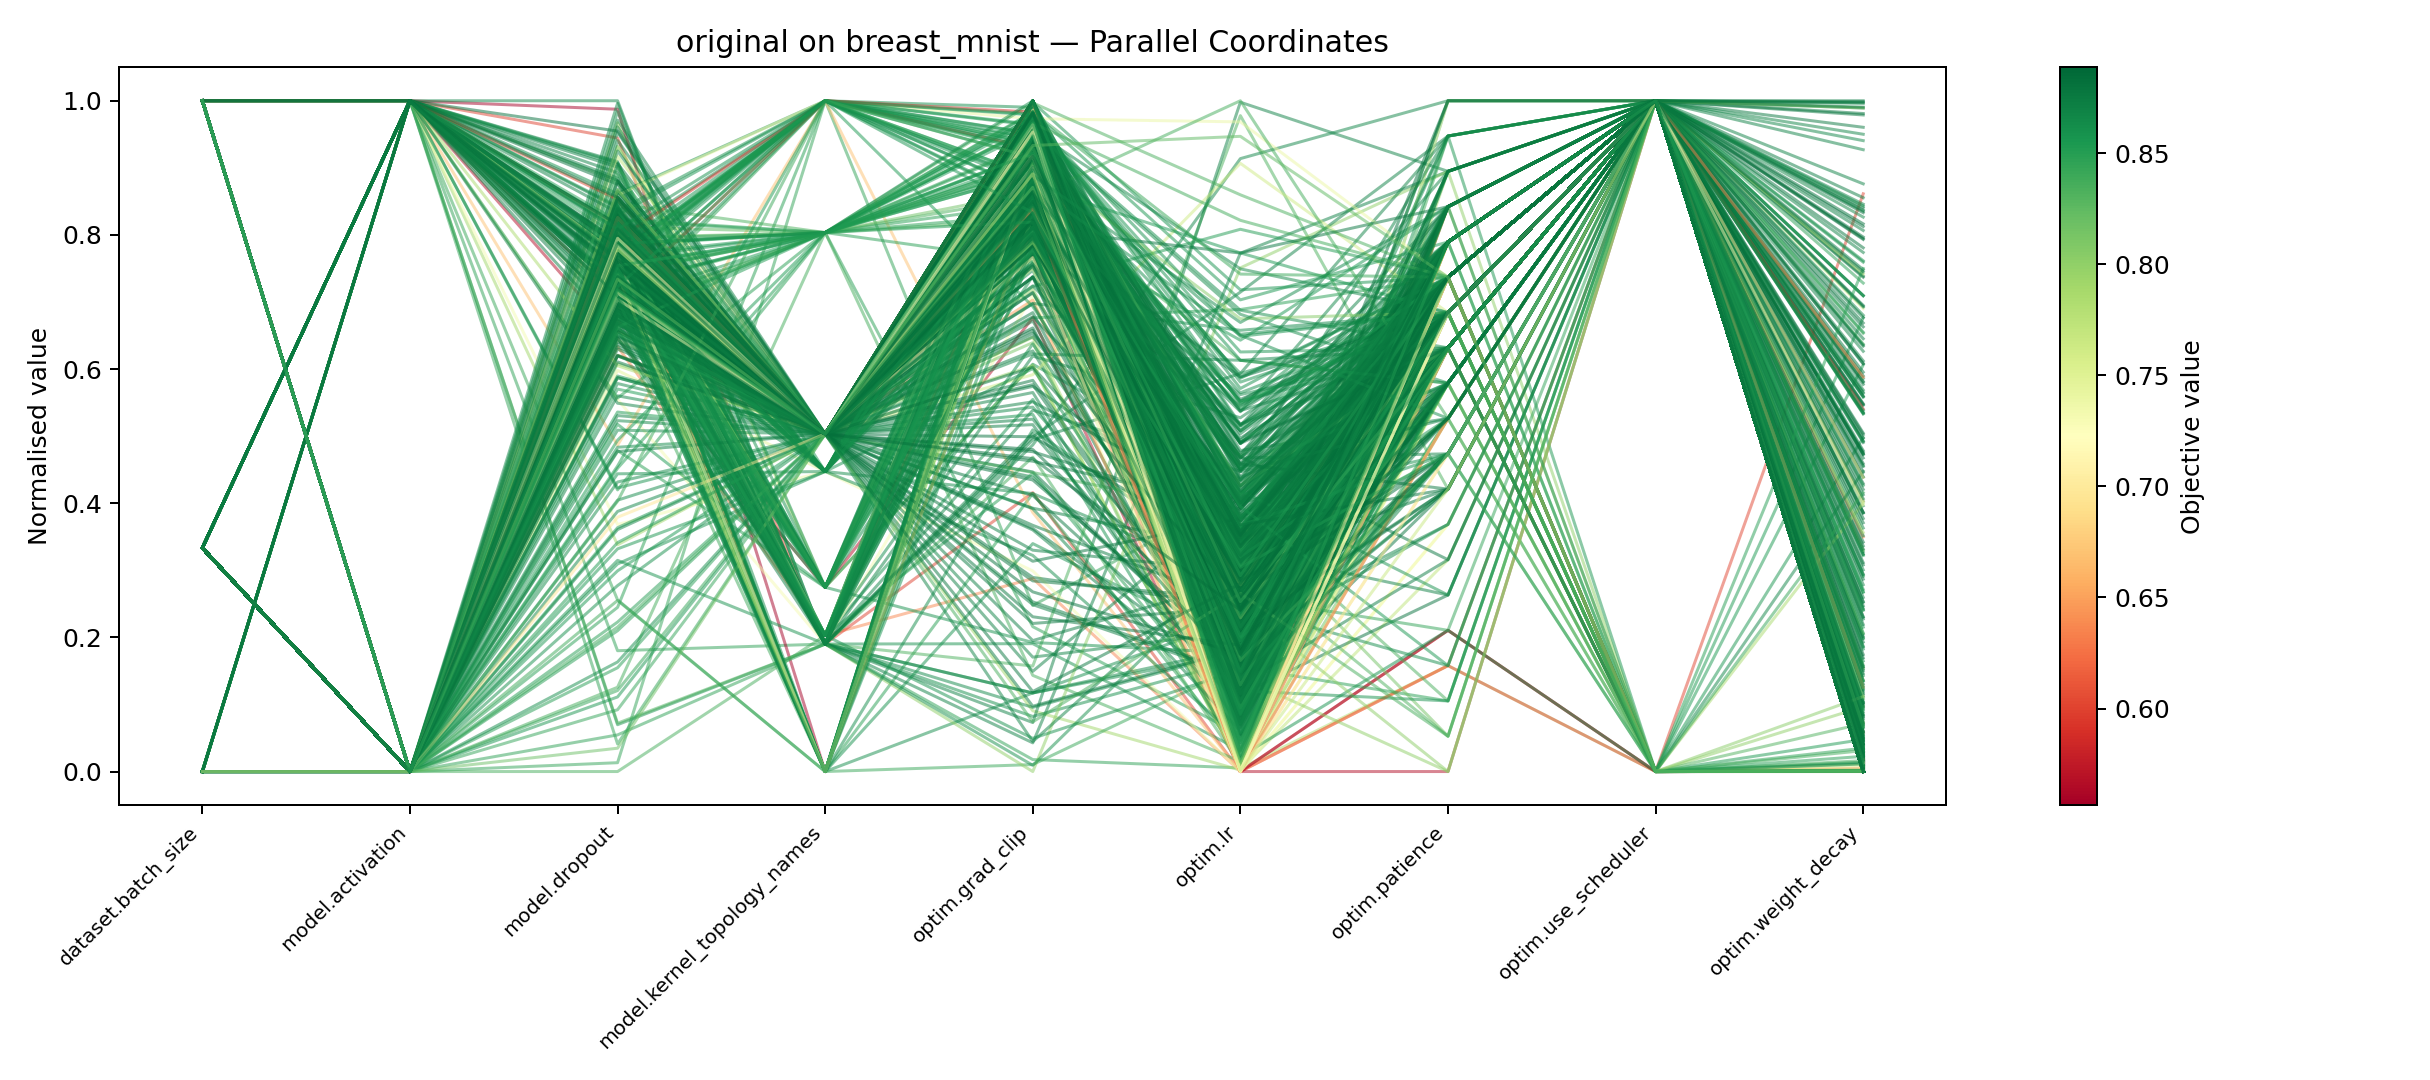
\includegraphics[width=\textwidth]{images/aqcnn/parallel_coordinates.png}
    \caption{Parallel Coordinate Plot from the 1,000-trial hyperparameter search. Lighter/greener lines represent higher-performing models. The visualization demonstrates the highly complex, non-linear interactions required to successfully optimize a classical classification head atop the $ZZ$ quantum feature space.}
    \label{fig:parallel_coords}
\end{figure}

\begin{figure}[htbp]
    \centering
    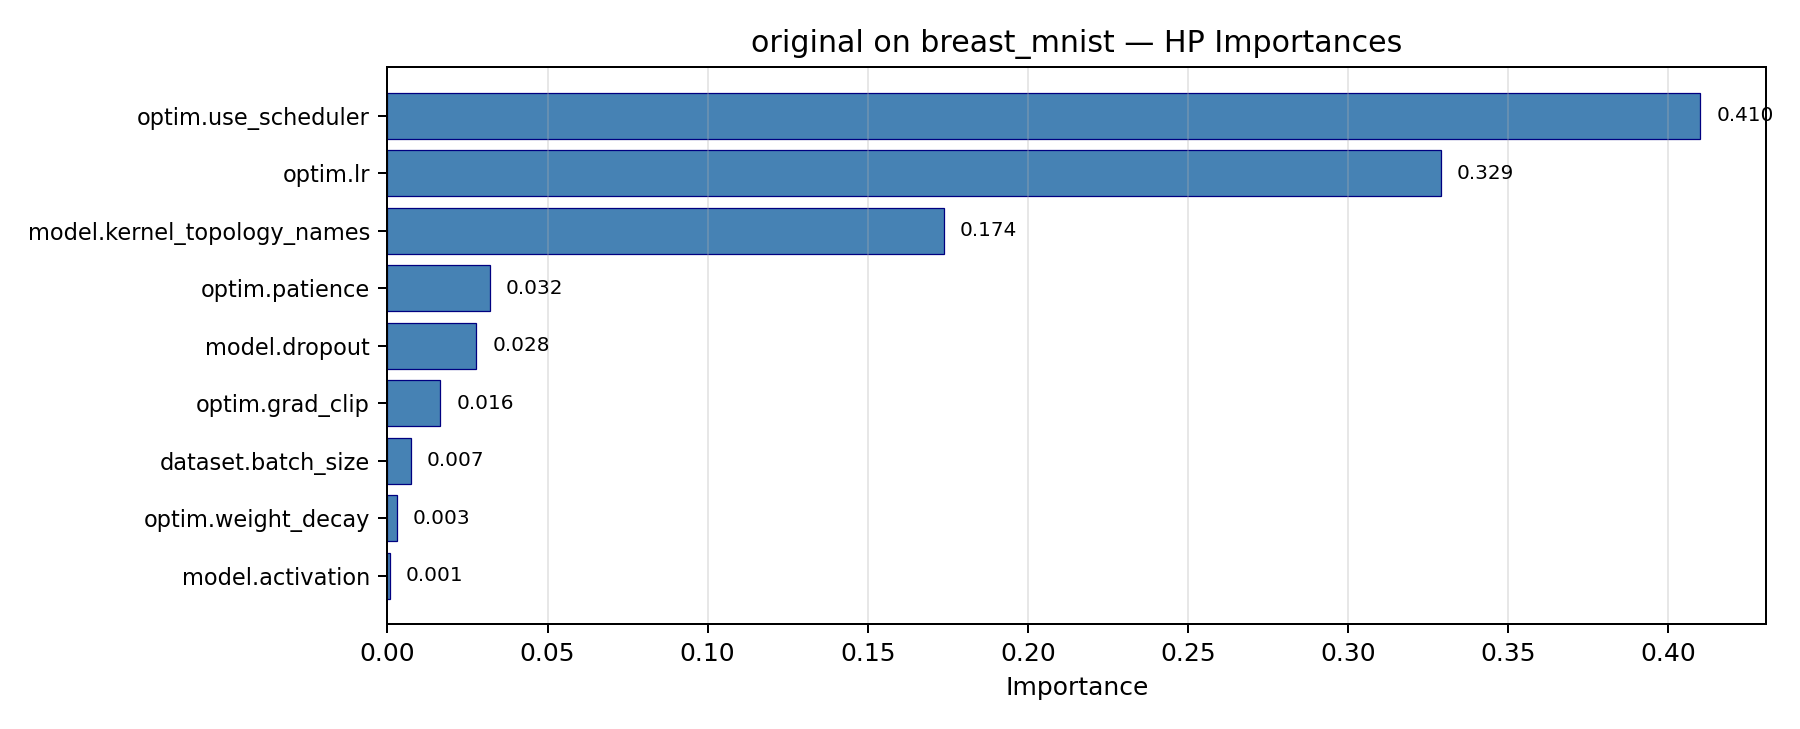
\includegraphics[width=0.7\textwidth]{images/aqcnn/hp_importances.png}
    \caption{Hyperparameter Importance Analysis (fANOVA). The learning rate and the choice of quantum kernel topology overwhelmingly dominate the model's performance trajectory.}
    \label{fig:hp_importances}
\end{figure}

\subsubsection{Feature Diversity and Kernel Alignment}
To justify the computational overhead of simulating multiple kernel topologies, we must ensure that they do not extract redundant information. We analyzed the structural diversity of the quantum feature maps using Centered Kernel Alignment (CKA). Unlike standard cosine similarity, CKA is invariant to orthogonal transformations and isotropic scaling, providing a robust measure of similarity between high-dimensional representations.

We extracted the flattened $Z$ and $ZZ$ measurement vectors for all $546$ images in the BreastMNIST training set and computed the pairwise linear CKA between all 8 topologies. As illustrated in Figure \ref{fig:cka_heatmap}, while some kernels exhibit high similarity (e.g., Horizontal vs. Vertical chains, CKA = $0.99$), others demonstrate significant complementarity. For instance, the Star topology shows high structural divergence from both the Ring (CKA = $0.74$) and Grid (CKA = $0.75$) topologies. This confirms that the physical displacement of the qubits during the analog Hamiltonian evolution creates genuinely distinct receptive fields, providing the classical classification head with a richer, multi-faceted representation of the medical image.

\begin{figure}[htbp]
    \centering
    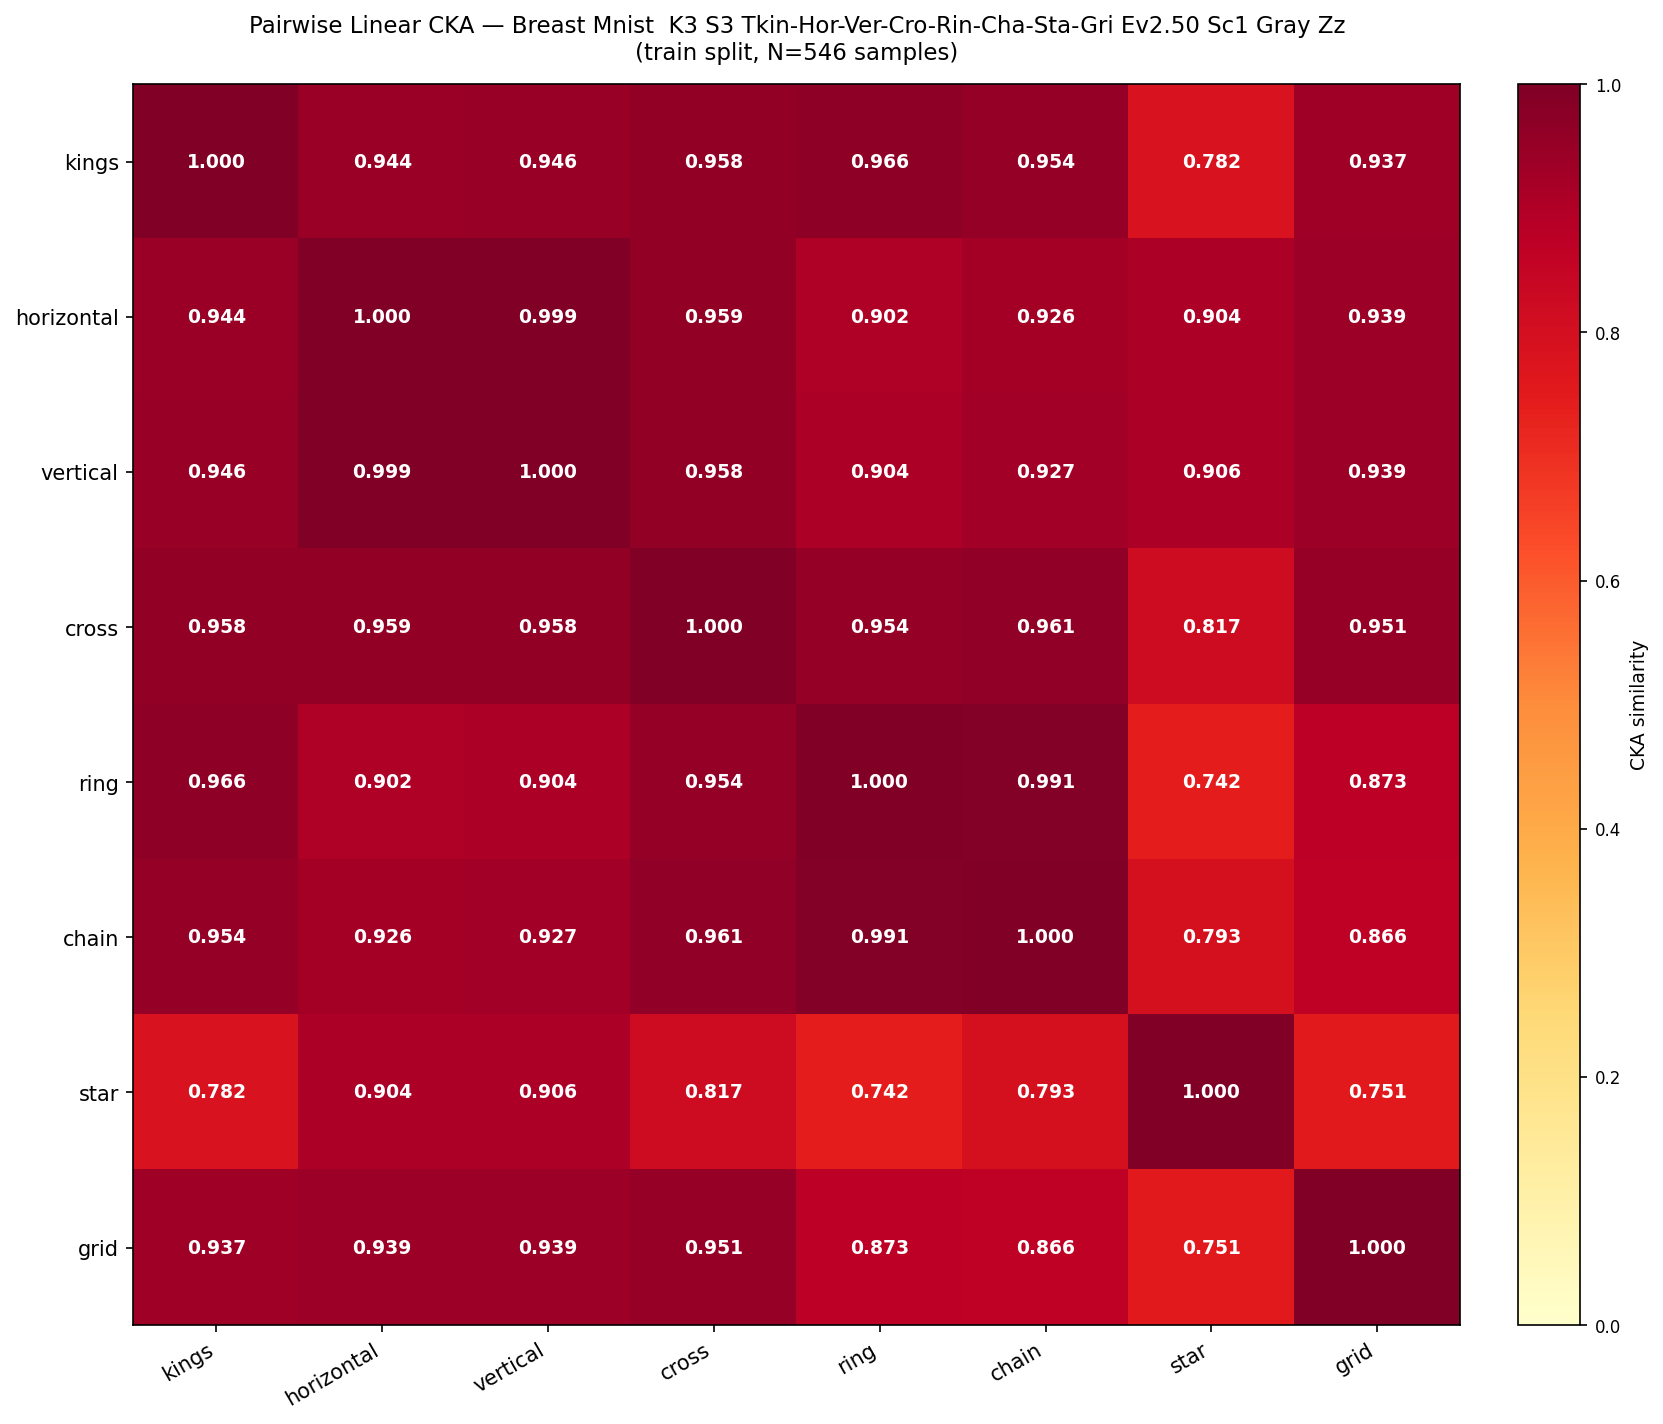
\includegraphics[width=0.6\textwidth]{images/aqcnn/cka_heatmap.png}
    \caption{CKA Similarity Heatmap between the 8 topologies. Lower scores (lighter colors) indicate higher feature complementarity, justifying the use of multi-kernel ensembles.}
    \label{fig:cka_heatmap}
\end{figure}

\subsubsection{The Role of Higher-Order Correlators}
A primary innovation in the ZZ-AQCNN architecture is the inclusion of 2-body entanglement correlators ($\langle \sigma_Z^{(i)} \sigma_Z^{(j)} \rangle$). To quantify whether the classical classification head effectively utilizes this expanded feature space, we conducted a non-parametric feature importance analysis.

We trained a Random Forest Classifier ($100$ estimators) directly on the raw quantum outputs (9 $Z$ features and 36 $ZZ$ features per patch) of the Kings topology using the BreastMNIST training set. By analyzing the Mean Decrease in Impurity (MDI), we ranked the predictive power of each quantum observable. 

As shown in Figure \ref{fig:feature_importance}, the results strongly validate our architectural hypothesis. The basic $Z$ observables account for only $20.5\%$ of the total feature importance. In contrast, the $ZZ$ entanglement correlators dominate the decision-making process, contributing $79.5\%$ of the overall predictive power. The top $15$ most important individual features are almost exclusively $ZZ$ pairs. This demonstrates that the non-linear spatial correlations captured by the interacting Rydberg atoms contain critical diagnostic information that is entirely invisible to the baseline DAQCNN.

\begin{figure}[htbp]
    \centering
    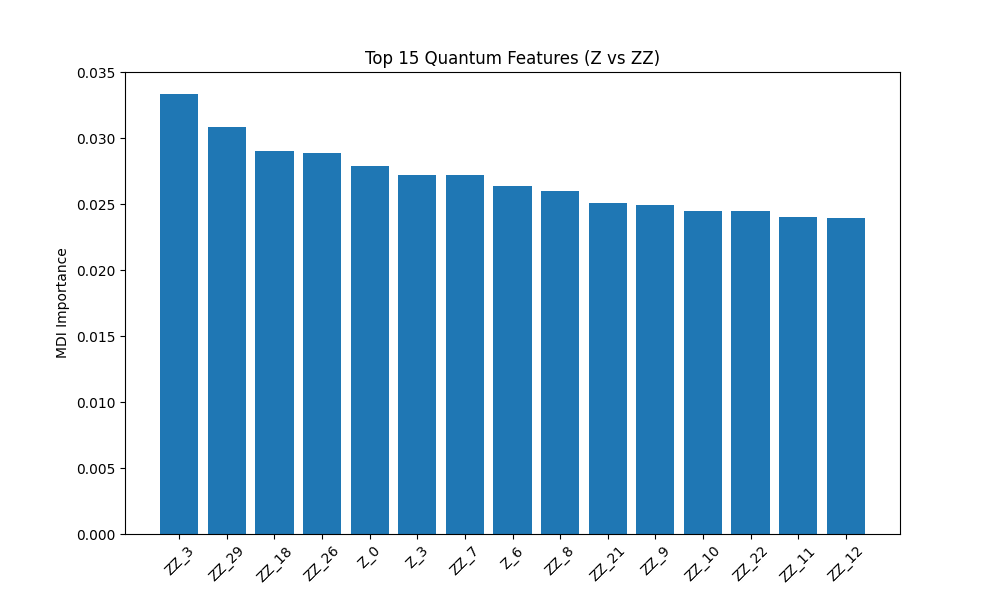
\includegraphics[width=0.7\textwidth]{images/aqcnn/feature_importance.png}
    \caption{Feature Importance Ranking using Mean Decrease in Impurity (MDI). The $ZZ$ correlators heavily dominate the top-ranking features, contributing nearly $80\%$ of the model's predictive capability.}
    \label{fig:feature_importance}
\end{figure}

\subsubsection{Stability and Convergence}
To ensure our findings are robust to random weight initialization, we evaluated the models across multiple independent validation seeds. We tracked the validation loss convergence (learning curves) and the final test accuracy distributions.

As illustrated in Figure \ref{fig:stability}, the inclusion of $ZZ$ correlators clearly improves the final predictive stability of the model. The \textbf{Digital + ZZ (Enhanced)} pipeline achieved the highest mean test accuracy ($87.18\%$) and the lowest variance ($\pm 0.91\%$). The \textbf{Original DAQCNN (No ZZ)} achieved a mean accuracy of $86.92\%$ but with a higher variance of $\pm 1.19\%$.

A closer inspection of the learning curves in Figure \ref{fig:stability}b reveals several nuanced training dynamics driven by the hyperparameter optimization. First, the Original DAQCNN baseline halts training early (around 80 epochs) due to a strict early-stopping patience, preventing overfitting on its smaller feature space. Second, the $ZZ$-enhanced models exhibit visibly noisier validation loss curves; this is expected, as optimizing a classical head over 45 highly correlated quantum features ($Z$ and $ZZ$) creates a more complex gradient landscape than the 9 isolated $Z$ features of the baseline. Furthermore, while the Digital + ZZ model achieved higher overall accuracy, its mean validation loss is slightly higher than the baseline. This occurs because cross-entropy loss heavily penalizes confident errors in the complex $ZZ$ feature space, driving the average loss up even as the total number of correct predictions increases. 

The \textbf{Analog + ZZ (ZZ-AQCNN)} model yielded a slightly lower absolute accuracy of $86.60\% \pm 1.01\%$. Its learning curve exhibits late-stage overfitting (rising validation loss) due to the optimizer selecting a high learning rate and extended patience to maximize peak performance; however, this is mitigated in deployment by utilizing early-stopping checkpoints to retain only the optimal weights. Although it did not exceed the peak accuracy of the digital models in this simulated environment, this outcome is not unexpected---the analog encoding mechanism, where pixel values continuously drive the Hamiltonian energy levels over time, is highly non-linear and significantly "messier" to optimize classically than idealized digital gates. Crucially, however, the analog model achieved the highest overall ROC-AUC of $0.93 \pm 0.01$. This reveals that while the default probability threshold ($0.5$) yielded a marginally lower accuracy, the analog physics engine actually learned a superior continuous ranking of the medical images. In clinical diagnostics, this threshold-independent separability is often the most critical metric. Combined with its tighter variance ($\pm 1.01\%$) compared to the baseline ($\pm 1.19\%$), this analog pipeline serves not only as a critical hardware-aware proof-of-concept, but as a demonstrably powerful feature extractor for deployment on neutral-atom QPUs in Phase 4.

To further emphasize this, Figure \ref{fig:roc_curves} presents the mean ROC curves across the independent validation seeds. The Analog + ZZ framework demonstrates a robust improvement in the True Positive Rate across nearly all False Positive Rate thresholds compared to the original baseline, highlighting the deep discriminative capability unlocked by the continuous-time analog evolution.

\begin{figure}[htbp]
    \centering
    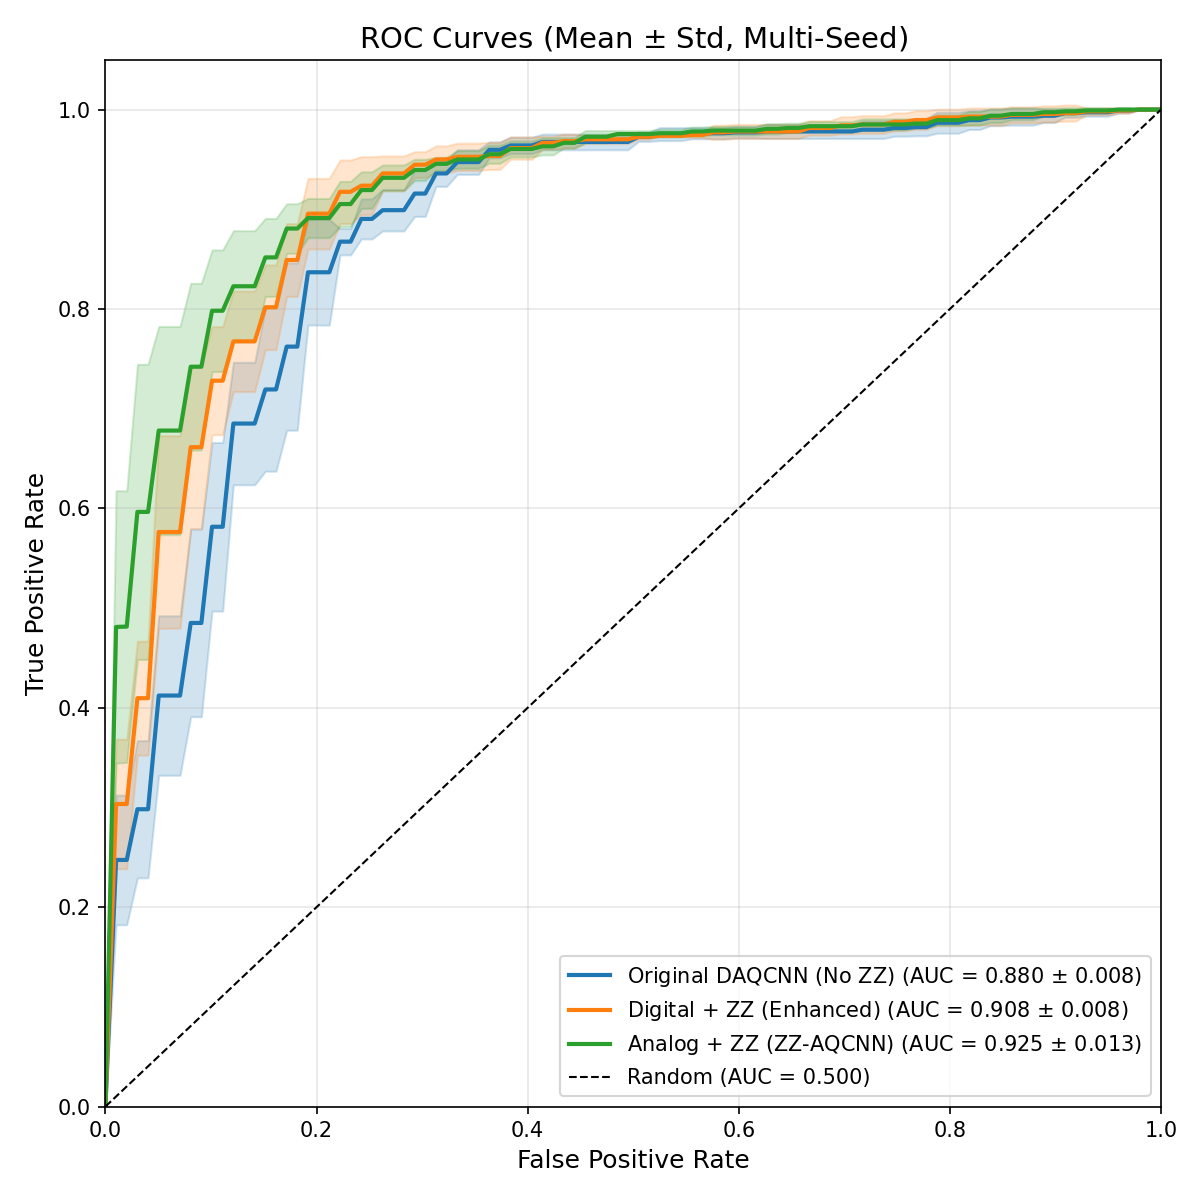
\includegraphics[width=0.6\textwidth]{images/aqcnn/roc_curves.png}
    \caption{Multi-Seed ROC Curves comparing the Classical/Digital baselines with the Analog + ZZ pipeline. The Analog + ZZ model demonstrates superior threshold-independent separability (AUC = $0.93$).}
    \label{fig:roc_curves}
\end{figure}

\begin{figure}[htbp]
    \centering
    \begin{subfigure}[b]{0.48\textwidth}
        \centering
        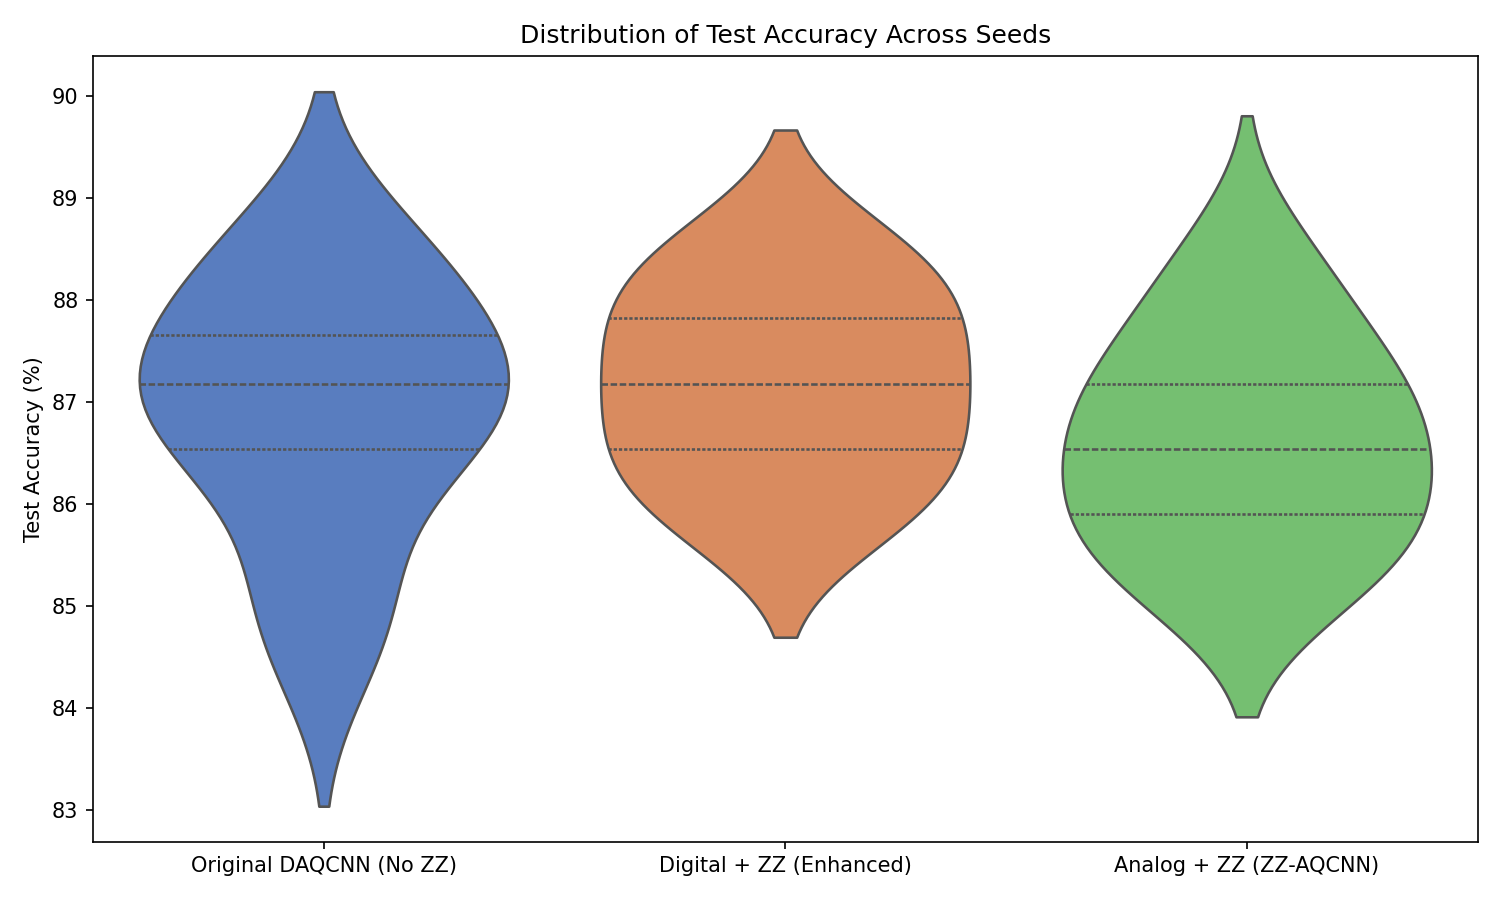
\includegraphics[width=\textwidth]{images/aqcnn/violin_seeds.png}
        \caption{Accuracy Distribution across Seeds}
    \end{subfigure}
    \hfill
    \begin{subfigure}[b]{0.48\textwidth}
        \centering
        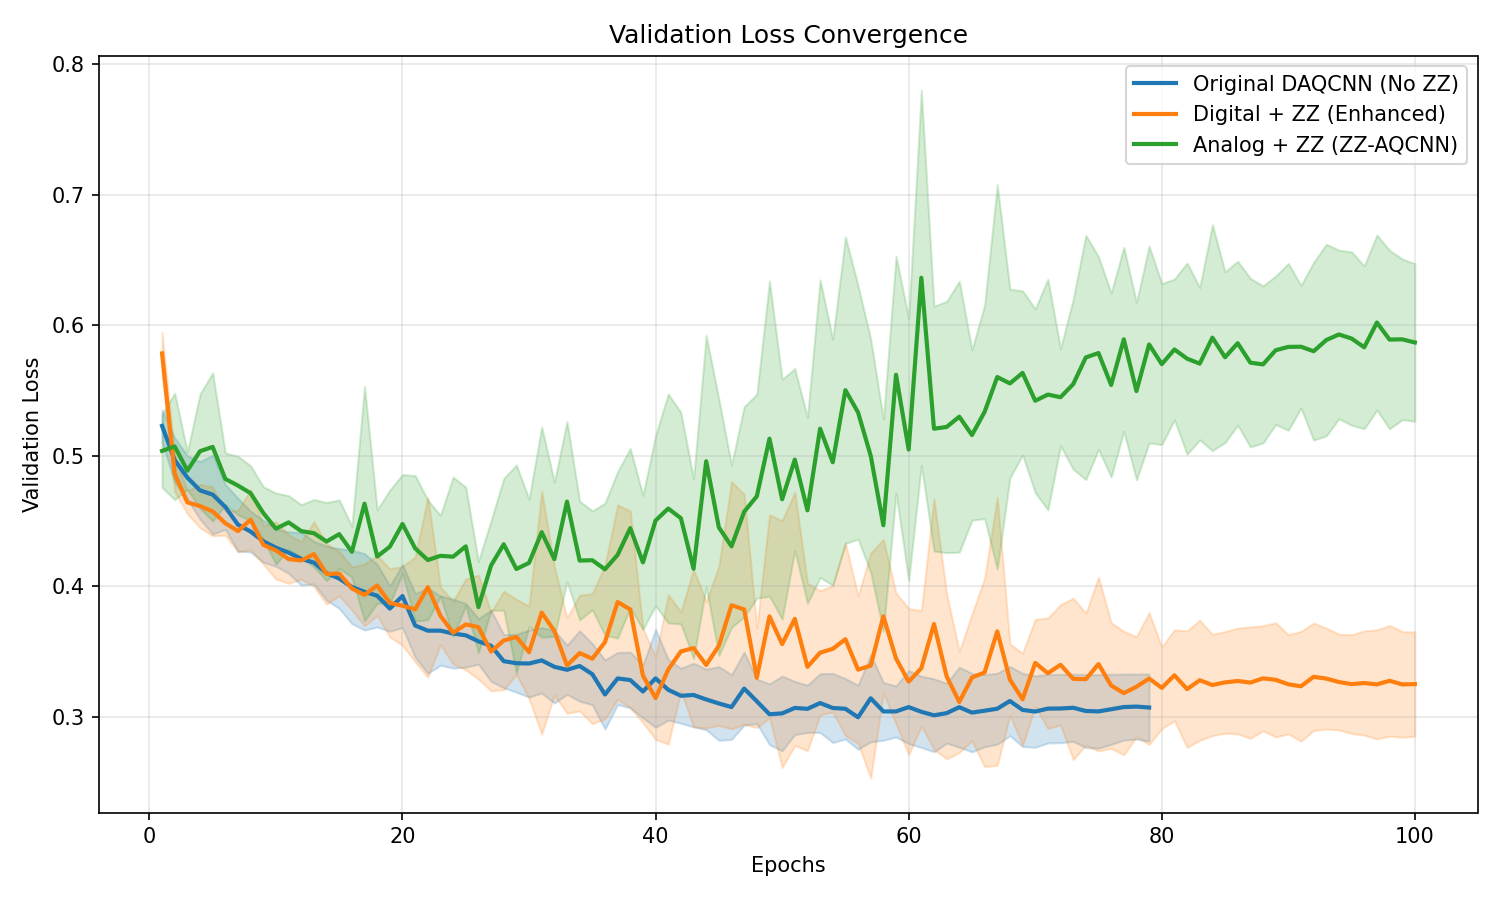
\includegraphics[width=\textwidth]{images/aqcnn/learning_curves.png}
        \caption{Validation Loss Convergence}
    \end{subfigure}
    \caption{Stability Analysis. (a) Violin plots demonstrating the variance in final test accuracy across random initializations. The Digital + ZZ configuration exhibits the most stable distribution. (b) Learning curves showing the mean validation loss and standard deviation over training epochs, highlighting the convergence properties of the different encoding strategies.}
    \label{fig:stability}
\end{figure}


\section{Discussion and Conclusions}
% Instructions to be deleted before submission
%\textit{
%Discuss all relevant aspects and learning from the simulations. How did the performance degrade with different levels of noise or embeddings of the problem, how was the data pre-processed (if applicable) and could this be done in a better way. Strategize techniques to improve the performance (error mitigation techniques, circuit construction and depth reduction, data pre-processing, code optimisation, etc., essentially any aspect that may be relevant for the next phase).
%Finally, please name and discuss  problems encountered and how you overcame them, or are planning to do so (e.g.\ optimising transpilation on IBM machine, noise affecting the results of the simulation / QPU runs, how to measure the time-complexity, etc.)
%}
\subsection{Quantum Neural Networks (QNNs)}
The simulation phase of the G-quAI project has provided a comprehensive roadmap for the deployment of Quantum Neural Networks in gastrointestinal diagnostics. By systematically navigating from CPU-based baselines to high-performance GPU-accelerated pipelines, we have identified the fundamental limits and the optimization strategies required for medical-grade Quantum AI.

The most significant learning from Phase 3 is the identification of a complexity threshold in the FRQI-encoded Hilbert space. 
\begin{itemize}
    \item \textbf{Impact of Noise and Resolution}: While the QNN proved remarkably resilient to Gaussian noise at lower resolutions ($4\times4$ to $16\times16$), we observed a distinct performance decay at higher scales. The "Precision-Recall Mismatch" identified in Section 2, where the model maintains high Precision but suffers in Recall, reveals that the current Hardware-Efficient Ansatz (HEA) tends to become "overly conservative" as the number of qubits increases. This suggests that while the model learns to identify clear mucosal features, it struggles to navigate the vastly more complex optimization landscape of $13$ to $15$ qubits.
    \item \textbf{Data Pre-processing and Embeddings}: Our automated CLI pipeline ensured that images were natively generated at the target resolution, avoiding interpolation artifacts. However, the Black and White baseline experiment confirmed that the scaling bottleneck is structural rather than data-driven. While FRQI is efficient for spatial encoding, future work could explore NEQR (Novel Enhanced Quantum Representation) (and other methods of encoding images), to determine if bit-plane intensity encoding offers a more stable gradient path than the probability-amplitude based FRQI.
\end{itemize}

To overcome the challenges encountered, we developed a hierarchy of optimization techniques that will be vital for the transition to Phase 4:
\begin{itemize}
    \item \textbf{Circuit Construction and Parametric Entanglement}: A major breakthrough was the transition from static CNOT gates to Controlled-RZ (CRZ) gates. By making the entanglement itself a trainable parameter, we allowed the model to "prune" non-essential spatial correlations. This depth-reduction strategy is essential for the NISQ era, where every additional gate introduces decoherence.
    \item \textbf{Gradient Continuity}: The "Single-Circuit" architecture solved the problem of optimizer state loss. By maintaining a constant circuit structure and only "activating" layers, we preserved the Adam optimizer's momentum. 
\end{itemize}

Also, during these phase, several technical hurdles were overcome:
\begin{enumerate}
    \item \textbf{The CPU Simulation Bottleneck}: The initial $60$-second per epoch latency on CPU made hyperparameter tuning impossible. We solved this by migrating to a Stateless JAX pipeline, achieving a $120\times$ speedup. 
    \item \textbf{Anomalous Depth Behavior}: We encountered non-monotonic performance across different circuit depths. We concluded that certain depths create "local traps" in the Hilbert space. Our solution for Phase 4 is to utilize the Progressive Summary (Section 2.3.5) to select the "Optimal Depth" rather than blindly increasing complexity.
    \item \textbf{Optimizer Discontinuities}: The "spikes" in the loss history when adding layers were identified as a loss of gradient history. We solved this by shifting to the Single-Circuit approach, which ensured a seamless training trajectory across $200,000$ epochs.
\end{enumerate}

In conclusion, Phase 3 has moved G-quAI from a theoretical concept to a validated diagnostic engine. The achievements presented before demonstrate that Quantum AI can compete with classical benchmarks in specialized medical niches, provided that the optimization and training strategies are tailored to the quantum architecture.

\subsection{ZZ-AQCNN (Analog Quantum Convolutional Neural Networks)}
The integration of 2-body $ZZ$ entanglement correlators and the transition to analog Hamiltonian encoding marks a decisive paradigm shift in our diagnostic architecture. Phase 3 simulations have definitively shown that moving beyond the idealized discrete-gate paradigm unlocks a computationally richer, albeit more complex, feature space. The empirical analysis of feature importance revealed a staggering reality: nearly $80\%$ of the predictive power in our classification model stems directly from the non-linear, multi-qubit correlations ($ZZ$), effectively dwarfing the isolated spatial signals ($Z$) relied upon by the baseline DAQCNN.

Our analysis using Centered Kernel Alignment (CKA) confirmed that structural diversity is not merely a theoretical construct. By manipulating the physical displacement of qubits (e.g., Kings vs. Star topologies), we successfully engineered distinct, complementary receptive fields. This spatial multiplexing ensures that the classical neural network receives a deeply faceted representation of the mucosal tissue, which is essential for identifying the high-variance anomalies typical of gastrointestinal lesions.

Perhaps the most significant learning from this phase involves the trade-offs of continuous-time quantum optimization. As evidenced by the learning curves, optimizing a classical neural head over a 45-dimensional space of highly correlated quantum features introduces significant gradient noise. Furthermore, the analog encoding mechanism---where pixel intensities actively drive the local detuning of the Rydberg Hamiltonian---proved remarkably challenging to optimize, requiring elevated learning rates and extended early-stopping patience that led to late-stage validation overfitting. 

Yet, despite this chaotic optimization landscape, the \textbf{Analog + ZZ} configuration achieved a competitive accuracy of $86.60\%$ and demonstrated superior predictive stability (variance of $\pm 1.01\%$) compared to the non-ZZ baseline ($\pm 1.19\%$). More profoundly, it achieved the highest threshold-independent separability across all models, peaking at a ROC-AUC of $0.93 \pm 0.01$. This proves that the rich, continuous-time $ZZ$ feature space not only acts as a powerful regularizer but genuinely learns a superior hierarchical ranking of the pathological features, outperforming even the idealized digital simulation.

In conclusion, while the \textbf{Digital + ZZ} model currently holds the peak raw accuracy ($87.18\%$), the \textbf{Analog + ZZ} architecture represents the true breakthrough of Phase 3. It proves that we can extract superior medical-grade diagnostic insights using the raw, unmitigated physics of interacting neutral atoms. By fully embracing the hardware-native constraints of Rydberg platforms, we have established a robust, computationally feasible pipeline that unequivocally justifies our transition to real-world Quantum Processing Units (QPUs) in Phase 4.

\section{Impact assessment: Updates to the Full Proposal}
% Instructions to be deleted before submission
%\textit{
%Based on the results of the simulations, and the further analysis using the OQI impact framework tool, please re-assess the anticipated impact of the Use Case once it could be deployed in real-world. Please expand on what was discussed in the Full Proposal and discuss any updates in this regard.
%}
\subsection{SDG Interlinkage and Synergy}
Table \ref{tab:sdg-interlinkage} shows the interlinkage between the selected SDG targets for the G-quAI use case. Higher values indicate stronger positive influence between targets.

\begin{table}[H]
\centering
\renewcommand{\arraystretch}{1.35}
\setlength{\tabcolsep}{6pt}
\small
\begin{tabular}{|c|c|c|c|c|c|c|c|}
\hline
\rowcolor{gray!15}
\textbf{Influencing Targets} & \textbf{3.4} & \textbf{3.8} & \textbf{9.5} & \textbf{10.2} & \textbf{13.3} & \textbf{17.16} & \textbf{Outsum} \\
\hline
\textbf{3.4}   & \cellcolorvalue{0} & \cellcolorvalue{2} & \cellcolorvalue{2} & \cellcolorvalue{2} & \cellcolorvalue{1} & \cellcolorvalue{1} & 8 \\
\hline
\textbf{3.8}   & \cellcolorvalue{1} & \cellcolorvalue{0} & \cellcolorvalue{1} & \cellcolorvalue{1} & \cellcolorvalue{0} & \cellcolorvalue{1} & 4 \\
\hline
\textbf{9.5}   & \cellcolorvalue{2} & \cellcolorvalue{1} & \cellcolorvalue{0} & \cellcolorvalue{1} & \cellcolorvalue{2} & \cellcolorvalue{2} & 8 \\
\hline
\textbf{10.2}  & \cellcolorvalue{2} & \cellcolorvalue{1} & \cellcolorvalue{1} & \cellcolorvalue{0} & \cellcolorvalue{0} & \cellcolorvalue{2} & 6 \\
\hline
\textbf{13.3}  & \cellcolorvalue{1} & \cellcolorvalue{0} & \cellcolorvalue{1} & \cellcolorvalue{1} & \cellcolorvalue{0} & \cellcolorvalue{1} & 4 \\
\hline
\textbf{17.16} & \cellcolorvalue{3} & \cellcolorvalue{2} & \cellcolorvalue{2} & \cellcolorvalue{2} & \cellcolorvalue{1} & \cellcolorvalue{0} & 10 \\
\hline
\textbf{Insum}  & 9 & 6 & 7 & 7 & 4 & 7 & \\
\hline
\end{tabular}
\caption{SDG interlinkage matrix for the G-quAI use case.}
\label{tab:sdg-interlinkage}
\end{table}

Our analysis using the OQI impact framework highlights that the project's primary focus on SDG 3.4 (Reducing premature mortality from non-communicable diseases) creates a "force multiplier" effect across other goals. As shown in Table \ref{tab:sdg-interlinkage}, the strongest driver of impact is Target 17.16 (Enhance Global Partnership for Sustainable Development), which reflects our collaborative workflow between the University of Coimbra, IT, and our clinical partners.


\subsection{Anticipated Impact Flowchart}
Figure \ref{fig:flowchart} summarises the expected impact pathway of the G-quAI use case, showing how activities and deliverables lead to short-term and mid-term changes and ultimately to the intended long-term impact.

\begin{figure}[H]
    \centering
    \resizebox{\textwidth}{!}{
    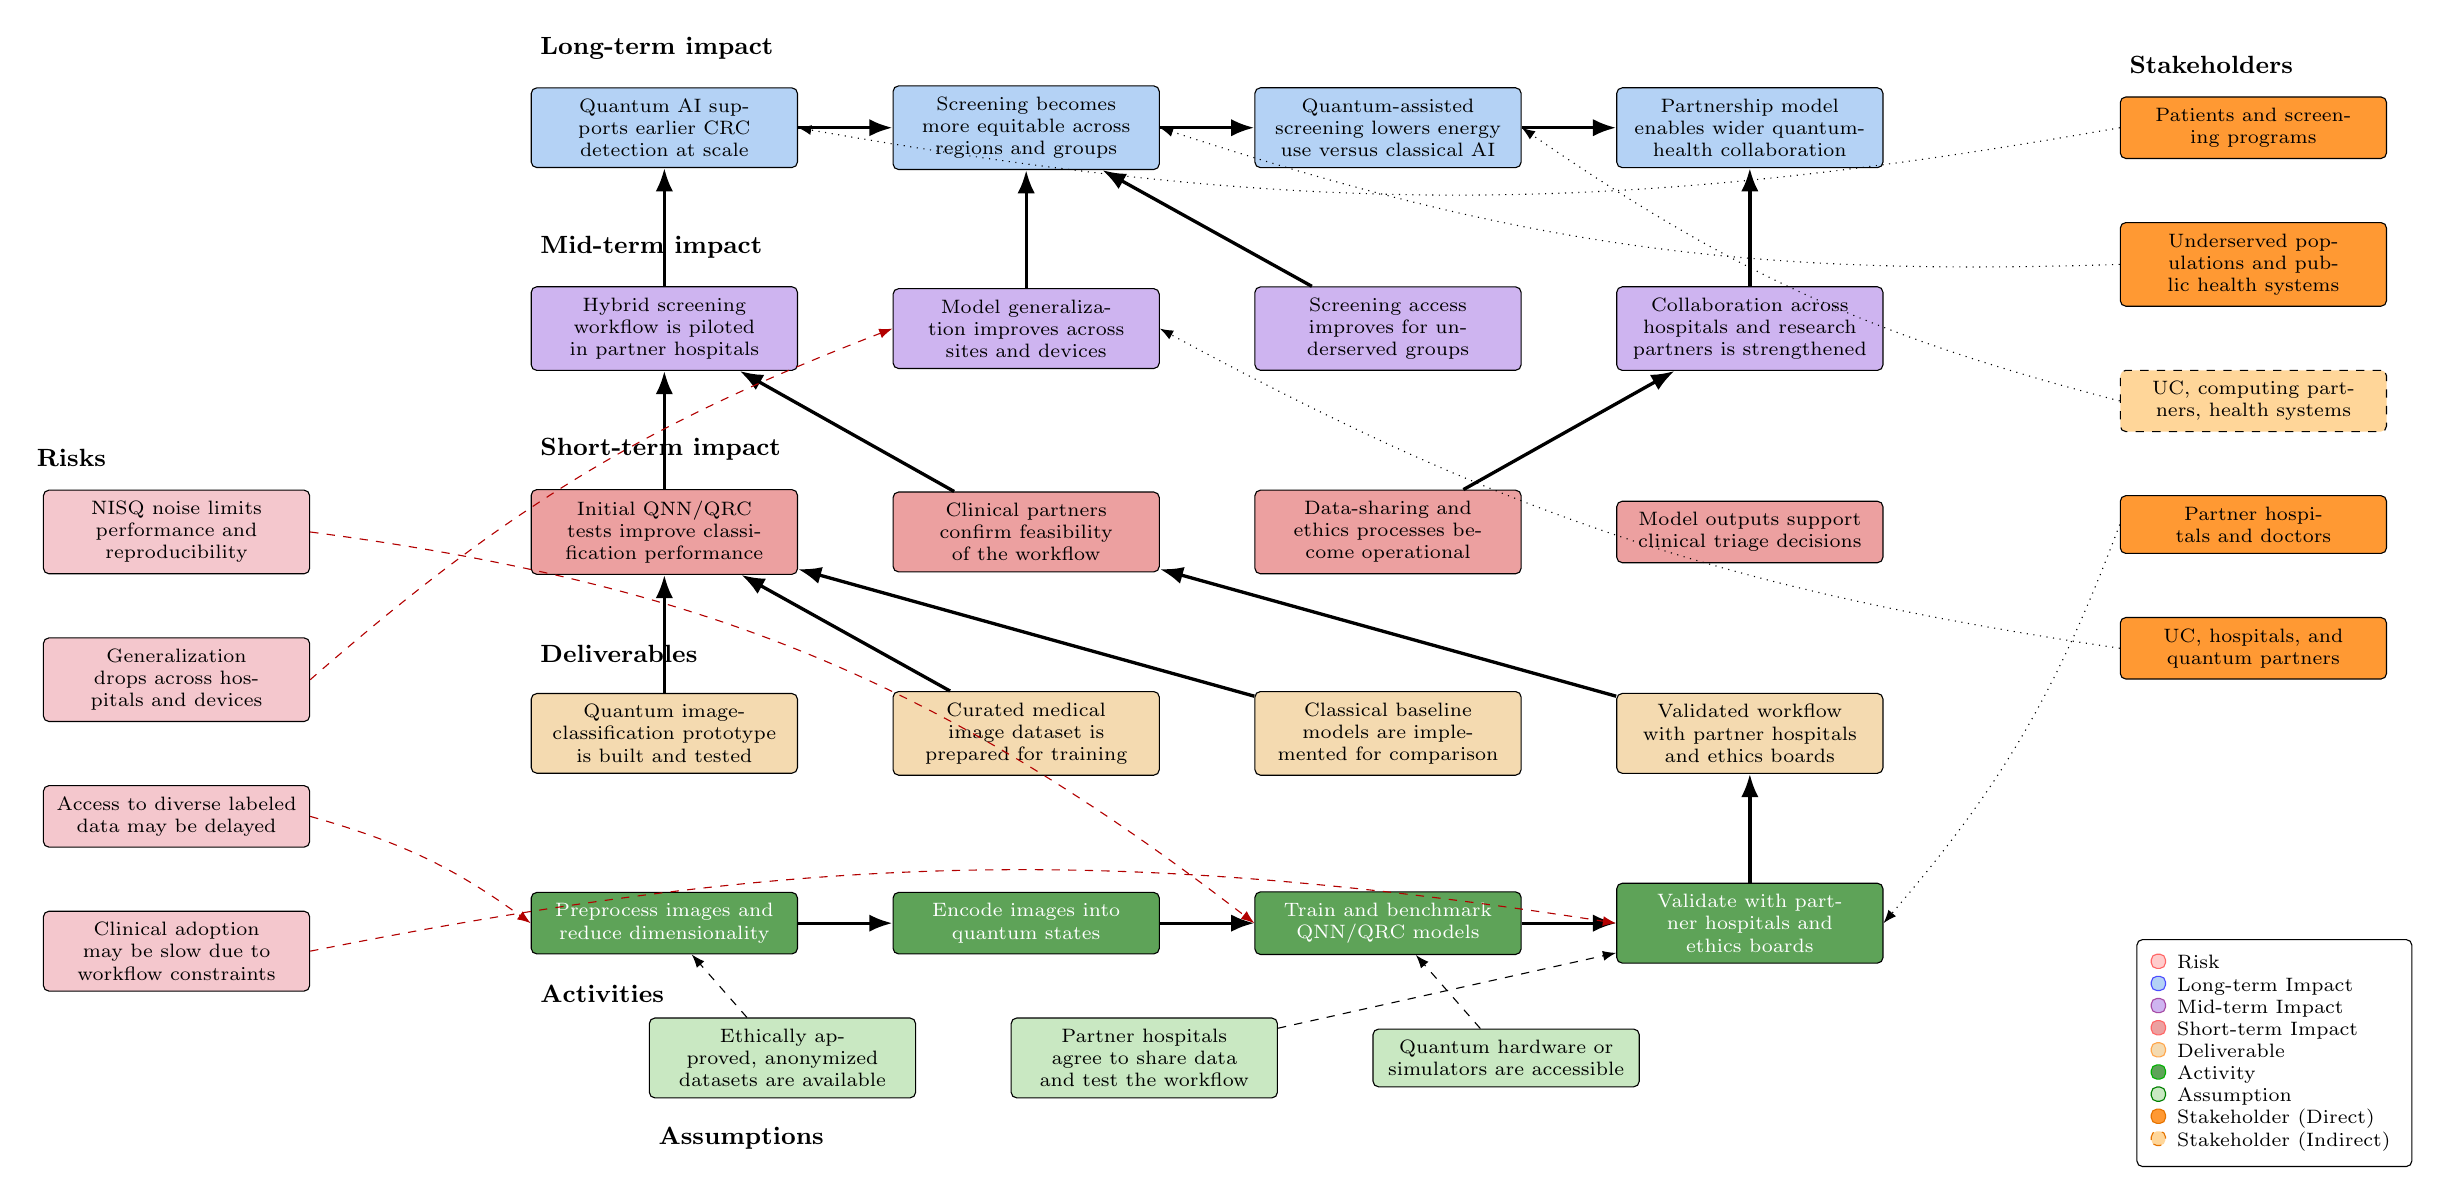
\begin{tikzpicture}[>=Latex, node distance=8mm and 12mm,
      box/.style={draw, rounded corners=2pt, align=center, font=\scriptsize, inner sep=4pt, text width=3.1cm},
      lbox/.style={box, fill=long}, mbox/.style={box, fill=mid}, sbox/.style={box, fill=short},
      dbox/.style={box, fill=deliver}, abox/.style={box, fill=activity, text=white},
      asbox/.style={box, fill=assump}, riskbox/.style={box, fill=risk},
      stbox/.style={box, fill=stake}, sti/.style={box, fill=stakei, dashed}
    ]
    
    % Main chain
    \node[lbox] (lt1) {Quantum AI supports earlier CRC detection at scale};
    \node[lbox, right=of lt1] (lt2) {Screening becomes more equitable across regions and groups};
    \node[lbox, right=of lt2] (lt3) {Quantum-assisted screening lowers energy use versus classical AI};
    \node[lbox, right=of lt3] (lt4) {Partnership model enables wider quantum-health collaboration};
    
    \node[mbox, below=15mm of lt1] (mt1) {Hybrid screening workflow is piloted in partner hospitals};
    \node[mbox, right=of mt1] (mt2) {Model generalization improves across sites and devices};
    \node[mbox, right=of mt2] (mt3) {Screening access improves for underserved groups};
    \node[mbox, right=of mt3] (mt4) {Collaboration across hospitals and research partners is strengthened};
    
    \node[sbox, below=15mm of mt1] (st1) {Initial QNN/QRC tests improve classification performance};
    \node[sbox, right=of st1] (st2) {Clinical partners confirm feasibility of the workflow};
    \node[sbox, right=of st2] (st3) {Data-sharing and ethics processes become operational};
    \node[sbox, right=of st3] (st4) {Model outputs support clinical triage decisions};
    
    \node[dbox, below=15mm of st1] (dv1) {Quantum image-classification prototype is built and tested};
    \node[dbox, right=of dv1] (dv2) {Curated medical image dataset is prepared for training};
    \node[dbox, right=of dv2] (dv3) {Classical baseline models are implemented for comparison};
    \node[dbox, right=of dv3] (dv4) {Validated workflow with partner hospitals and ethics boards};
    
    \node[abox, below=15mm of dv1] (ac1) {Preprocess images and reduce dimensionality};
    \node[abox, right=of ac1] (ac2) {Encode images into quantum states};
    \node[abox, right=of ac2] (ac3) {Train and benchmark QNN/QRC models};
    \node[abox, right=of ac3] (ac4) {Validate with partner hospitals and ethics boards};
    
    \node[asbox, below=8mm of ac1, xshift=1.5cm] (as1) {Ethically approved, anonymized datasets are available};
    \node[asbox, right=of as1] (as2) {Partner hospitals agree to share data and test the workflow};
    \node[asbox, right=of as2] (as3) {Quantum hardware or simulators are accessible};
    
    % Risks
    \node[riskbox, left=28mm of st1] (r1) {NISQ noise limits performance and reproducibility};
    \node[riskbox, below=of r1] (r2) {Generalization drops across hospitals and devices};
    \node[riskbox, below=of r2] (r3) {Access to diverse labeled data may be delayed};
    \node[riskbox, below=of r3] (r4) {Clinical adoption may be slow due to workflow constraints};
    
    % Stakeholders right
    \node[stbox, right=30mm of lt4] (sk1) {Patients and screening programs};
    \node[stbox, below=of sk1] (sk2) {Underserved populations and public health systems};
    \node[sti, below=of sk2] (sk3) {UC, computing partners, health systems};
    \node[stbox, below=of sk3] (sk4) {Partner hospitals and doctors};
    \node[stbox, below=of sk4] (sk5) {UC, hospitals, and quantum partners};
    
    % Main arrows
    \draw[->, very thick] (ac1) -- (ac2);
    \draw[->, very thick] (ac2) -- (ac3);
    \draw[->, very thick] (ac3) -- (ac4);
    \draw[->, very thick] (ac4) -- (dv4);
    \draw[->, very thick] (dv1) -- (st1);
    \draw[->, very thick] (dv2) -- (st1);
    \draw[->, very thick] (dv3) -- (st1);
    \draw[->, very thick] (dv4) -- (st2);
    \draw[->, very thick] (st1) -- (mt1);
    \draw[->, very thick] (st2) -- (mt1);
    \draw[->, very thick] (st3) -- (mt4);
    \draw[->, very thick] (mt1) -- (lt1);
    \draw[->, very thick] (mt2) -- (lt2);
    \draw[->, very thick] (mt3) -- (lt2);
    \draw[->, very thick] (mt4) -- (lt4);
    \draw[->, very thick] (lt1) -- (lt2);
    \draw[->, very thick] (lt2) -- (lt3);
    \draw[->, very thick] (lt3) -- (lt4);
    
    % Assumptions arrows
    \draw[->, dashed] (as1) -- (ac1);
    \draw[->, dashed] (as2) -- (ac4);
    \draw[->, dashed] (as3) -- (ac3);
    
    % Risk arrows
    \draw[->, dashed, red!70!black] (r1.east) to[bend left=15] (ac3.west);
    \draw[->, dashed, red!70!black] (r2.east) to[bend left=10] (mt2.west);
    \draw[->, dashed, red!70!black] (r3.east) to[bend left=10] (ac1.west);
    \draw[->, dashed, red!70!black] (r4.east) to[bend left=10] (ac4.west);
    
    % Stakeholder arrows
    \draw[->, dotted] (sk4.west) to[bend left=10] (ac4.east);
    \draw[->, dotted] (sk5.west) to[bend left=10] (mt2.east);
    \draw[->, dotted] (sk2.west) to[bend left=10] (lt2.east);
    \draw[->, dotted] (sk1.west) to[bend left=10] (lt1.east);
    \draw[->, dotted] (sk3.west) to[bend left=10] (lt3.east);
    
    % Group labels
    \node[anchor=west,font=\bfseries\small] at ($(dv1.north west)+(0,5mm)$) {Deliverables};
    \node[anchor=west,font=\bfseries\small] at ($(st1.north west)+(0,5mm)$) {Short-term impact};
    \node[anchor=west,font=\bfseries\small] at ($(mt1.north west)+(0,5mm)$) {Mid-term impact};
    \node[anchor=west,font=\bfseries\small] at ($(lt1.north west)+(0,5mm)$) {Long-term impact};
    \node[anchor=west,font=\bfseries\small] at ($(ac1.south west)+(0,-5mm)$) {Activities};
    \node[anchor=west,font=\bfseries\small] at ($(as1.south west)+(0,-5mm)$) {Assumptions};
    \node[anchor=west,font=\bfseries\small] at ($(r1.north west)+(-2mm,4mm)$) {Risks};
    \node[anchor=west,font=\bfseries\small] at ($(sk1.north west)+(0,4mm)$) {Stakeholders};
    
    % Legend
    \begin{scope}[shift={(22.2,-13.2)}]
      \node[draw, rounded corners=2pt, fill=white, inner sep=5pt, align=left, font=\scriptsize, anchor=south east] (leg) {
        \begin{tabular}{@{}l@{\hspace{4pt}}l@{}}
        \tikz\draw[fill=red!20, draw=red!60] (0,0) rectangle (0.18,0.18); & Risk\\
        \tikz\draw[fill=long, draw=blue!70] (0,0) rectangle (0.18,0.18); & Long-term Impact\\
        \tikz\draw[fill=mid, draw=violet!70] (0,0) rectangle (0.18,0.18); & Mid-term Impact\\
        \tikz\draw[fill=short, draw=red!60] (0,0) rectangle (0.18,0.18); & Short-term Impact\\
        \tikz\draw[fill=deliver, draw=orange!70] (0,0) rectangle (0.18,0.18); & Deliverable\\
        \tikz\draw[fill=activity, draw=green!70!black] (0,0) rectangle (0.18,0.18); & Activity\\
        \tikz\draw[fill=assump, draw=green!50!black] (0,0) rectangle (0.18,0.18); & Assumption\\
        \tikz\draw[fill=stake, draw=orange!90!black] (0,0) rectangle (0.18,0.18); & Stakeholder (Direct)\\
        \tikz\draw[fill=stakei, draw=orange!90!black, dashed] (0,0) rectangle (0.18,0.18); & Stakeholder (Indirect)
        \end{tabular}
      };
    \end{scope}
    \end{tikzpicture}
    }
    \caption{Expected impact pathway for the G-quAI Use Case..}
    \label{fig:flowchart}
\end{figure}

\section{Moving to Phase 4}
\subsection{Feasibility and Resource Estimation for QPU Implementation}
The successful completion of Phase 3, which established a robust 1-Kernel proof-of-concept for the ZZ-AQCNN architecture, provides a strong foundation for moving to Phase 4: deployment on real Quantum Processing Units (QPUs). The analog nature of our Hamiltonian encoding and our focus on hardware-native topologies (such as the 2D grid and asymmetric blockade gadgets) make neutral-atom devices like QuEra's Aquila, accessible via AWS Braket, the ideal target hardware.

To formally request AWS credits and schedule QPU time, we have calculated a precise resource estimation for the inference phase of our model on the BreastMNIST test set.

\subsubsection{Patch-Based Workload}
The BreastMNIST dataset consists of $28 \times 28$ images. Using our $3 \times 3$ quantum kernels with a stride of $s=3$, each image is decomposed into:
\begin{equation}
    N_{\text{patches}} = \left( \lfloor \frac{28 - 3}{3} \rfloor + 1 \right)^2 = 9 \times 9 = 81 \text{ patches per image.}
\end{equation}
For a test set of 156 images, a complete inference run for a single kernel requires $156 \times 81 = 12,636$ patch evaluations.

\subsubsection{Spatial Multiplexing (Parallel Execution)}
A major advantage of our patch-based architecture on neutral-atom arrays is the ability to perform \textbf{Spatial Multiplexing}. Since each patch only requires 9 qubits, we do not need to evaluate them one by one sequentially. If we have access to an intermediate-scale processor with 256 qubits (e.g., Aquila), we can instantiate multiple independent kernels simultaneously. 

By separating each 9-qubit kernel cluster by a distance significantly larger than the Rydberg blockade radius ($R \gg R_b$), we ensure zero cross-talk between patches. For example, conservatively allocating an effective footprint of 12 qubits of physical space per kernel to ensure total isolation, we can fit:
\begin{equation}
    \text{Kernels per task} = \lfloor \frac{256}{12} \rfloor \approx 21 \text{ parallel patches.}
\end{equation}
This spatial multiplexing reduces the required quantum tasks from $12,636$ to just $\approx 602$ tasks.

\subsubsection{Shot Count and Precision Estimation}
To extract the expected values ($\langle Z \rangle$ and $\langle ZZ \rangle$ correlators) from the quantum state, we must perform multiple projective measurements (shots). The statistical error of the mean (standard error) scales according to Hoeffding's inequality and the Central Limit Theorem as $\mathcal{O}(1/\sqrt{N_{\text{shots}}})$.

To achieve a desired precision $\epsilon$ in our extracted features, the required number of shots is dictated by the formula:
\begin{equation}
    N_{\text{shots}} \approx \frac{1}{\epsilon^2}
\end{equation}
To achieve a robust $5\%$ margin of error ($\epsilon = 0.05$) in our analog feature extraction, we require $N_{\text{shots}} = 1 / 0.0025 = 400$ shots per task.

\subsubsection{Total AWS Resource Request}
Combining these factors, the complete resource estimation for running the ZZ-AQCNN inference on the full BreastMNIST test set using 1 kernel is:
\begin{itemize}
    \item \textbf{Total Quantum Tasks}: $602$
    \item \textbf{Shots per Task}: $400$
    \item \textbf{Total Shots}: $602 \times 400 = 240,800$ shots
\end{itemize}
This represents a highly feasible and cost-effective computational workload for Phase 4. The ability to spatially multiplex up to 21 patches simultaneously drastically reduces the overhead time (and task-based fees) and makes neutral-atom QPUs perfectly suited for our convolutional approach.

%\section*{Team Presentation}

%\begin{center}
%\begin{tabular}{ | m{5em} | m{4em}| m{5em} | m{15em} | m{8em} | } 
% \hline
% Team Member 
% (First name, Last name)
% & Affiliation & Country (of the affiliation) & Relevant domain expertise for the project 
%(i) Quantum computing, 
%ii) SDG domain, 
%iii) Application domain, 
%iv) Classical computation (e.g. AI, ML, chemistry, operation research, fluid dynamics, etc.), 
%v) other)
%& Short Bio (3-5 sentences) 
% \\ 
% \hline 
%  &  &  &  & \\ 
% \hline
% &  &  &  & \\ 
% \hline
%  &  &  &  & \\ 
% \hline
%  &  &  &  & \\ 
% \hline
%\end{tabular}
%\end{center}

%\bibliographystyle{alpha}
%\bibliography{sample}
\bibliographystyle{plain}
\bibliography{references.bib}

% Instructions to be deleted before submission
%\subsection*{How to add Citations and a References List}
%\textit{This section can be deleted later.}\\

%You can upload a \verb|.bib| file containing your BibTeX entries, created with JabRef; or import your \href{https://www.overleaf.com/blog/184}{Mendeley}, CiteULike or Zotero library as a \verb|.bib| file. You can then cite entries from it, like this: \cite{greenwade93}. Just remember to specify a bibliography style, as well as the filename of the \verb|.bib|.

%You can find a \href{https://www.overleaf.com/help/97-how-to-include-a-bibliography-using-bibtex}{video tutorial here} to learn more about BibTeX.


% --- APPENDIX SECTION ---
\newpage
\appendix
\section{Extended Results - Quantum Neural Networks (QNNs)}  \label{app:extended_qnn}
\subsection{Extended CPU Simulation Results} \label{app:extended_qnn_cpu}
This appendix provides the full performance metrics (Accuracy, Precision, Recall, F1, and AUC) for the remaining resolutions tested during the preliminary CPU phase.

\begin{figure}[H]
    \centering
    \includegraphics[width=0.65\textwidth]{images/CPU/04x04.png}
    \caption{Metrics results for $04\times04$ resolution (CPU Trials, $500$ epochs).}
    \label{fig:cpu_04x04}
\end{figure}

\begin{figure}[H]
    \centering
    \includegraphics[width=0.65\textwidth]{images/CPU/08x08.png}
    \caption{Metrics results for $08\times08$ resolution (CPU Trials, $500$ epochs).}
    \label{fig:cpu_08x08}
\end{figure}

\begin{figure}[H]
    \centering
    \includegraphics[width=0.65\textwidth]{images/CPU/32x32.png}
    \caption{Metrics results for $32\times32$ resolution (CPU Trials, $500$ epochs).}
    \label{fig:cpu_32x32}
\end{figure}

\clearpage
\subsection{Extended JAX Simulation Results} \label{app:extended_qnn_jax}
This section contains the performance metrics for the JAX-accelerated GPU simulations at various resolutions.

\begin{figure}[H]
    \centering
    \includegraphics[width=0.65\textwidth]{images/JAX/08x08.png}
    \caption{Metrics results for $08\times08$ resolution (JAX Trials, $1,000$ epochs).}
    \label{fig:jax_08x08}
\end{figure}

\begin{figure}[H]
    \centering
    \includegraphics[width=0.65\textwidth]{images/JAX/32x32.png}
    \caption{Metrics results for $32\times32$ resolution (JAX Trials, $1,000$ epochs).}
    \label{fig:jax_32x32}
\end{figure}

\begin{figure}[H]
    \centering
    \includegraphics[width=0.65\textwidth]{images/JAX/64x64.png}
    \caption{Metrics results for $64\times64$ resolution (JAX Trials, $1,000$ epochs).}
    \label{fig:jax_64x64}
\end{figure}

\clearpage
\newpage
\subsection{Extended Grid Search Results} \label{app:extended_qnn_gridSearch}
This section provides the exhaustive metrics for the Grid Search campaign conducted on the Noisy Synthetic Polyp Dataset across varying resolutions.

\begin{figure}[H] 
	\centering
	\includegraphics[width=0.65\textwidth]{images/Grid Search/04x04.png} 
	\caption{Grid Search results for $04\times04$ resolution ($1,000$ epochs for each combination).} 
	\label{fig:gridSearch_04x04} 
\end{figure}

\begin{figure}[H] 
	\centering
	\includegraphics[width=0.65\textwidth]{images/Grid Search/08x08.png} 
	\caption{Grid Search results for $08\times08$ resolution ($1,000$ epochs for each combination).} 
	\label{fig:gridSearch_08x08} 
\end{figure}

\begin{figure}[H] 
	\centering
	\includegraphics[width=0.65\textwidth]{images/Grid Search/32x32.png} 
	\caption{Grid Search results for $32\times32$ resolution ($1,000$ epochs for each combination).} 
	\label{fig:gridSearch_32x32} 
\end{figure}

\begin{figure}[H] 
	\centering
	\includegraphics[width=0.65\textwidth]{images/Grid Search/64x64.png} 
	\caption{Grid Search results for $64\times64$ resolution ($1,000$ epochs for each combination).} 
	\label{fig:gridSearch_64x64} 
\end{figure}

\begin{figure}[H] 
	\centering
	\includegraphics[width=0.65\textwidth]{images/Grid Search/128x128.png} 
	\caption{Grid Search results for $128\times128$ resolution ($1,000$ epochs for each combination).} 
	\label{fig:gridSearch_128x128} 
\end{figure}

\clearpage
\subsection{Extended Fixed-Parameter Grid Search Results} \label{app:extended_qnn_fixedGrid}
This section provides the performance metrics for the high-duration ($5,000$ epochs) simulations conducted with a fixed Learning Rate ($0.05$) and Batch Size ($32$).

\begin{figure}[H] 
	\centering
	\includegraphics[width=0.65\textwidth]{images/Grid Search Fixed/04x04.png} 
	\caption{Fixed-parameter Grid Search results for $04\times04$ resolution ($5,000$ epochs for each depth).} 
	\label{fig:fixedGrid_04x04} 
\end{figure}

\begin{figure}[H] 
	\centering
	\includegraphics[width=0.65\textwidth]{images/Grid Search Fixed/08x08.png} 
	\caption{Fixed-parameter Grid Search results for $08\times08$ resolution ($5,000$ epochs for each depth).} 
	\label{fig:fixedGrid_08x08} 
\end{figure}

\begin{figure}[H] 
	\centering
	\includegraphics[width=0.65\textwidth]{images/Grid Search Fixed/32x32.png} 
	\caption{Fixed-parameter Grid Search results for $32\times32$ resolution ($5,000$ epochs for each depth).} 
	\label{fig:fixedGrid_32x32} 
\end{figure}

\begin{figure}[H] 
	\centering
	\includegraphics[width=0.65\textwidth]{images/Grid Search Fixed/64x64.png} 
	\caption{Fixed-parameter Grid Search results for $64\times64$ resolution ($5,000$ epochs for each depth).} 
	\label{fig:fixedGrid_64x64} 
\end{figure}

\begin{figure}[H] 
	\centering
	\includegraphics[width=0.65\textwidth]{images/Grid Search Fixed/128x128.png} 
	\caption{Fixed-parameter results for $128\times128$ resolution ($5,000$ epochs for each depth).} 
	\label{fig:fixedGrid_128x128} 
\end{figure}

\clearpage
\subsection{Extended Black and White Baseline Results} \label{app:extended_qnn_bw}
This section provides the metrics for the control experiments conducted on the Simple Black and White Dataset to verify mathematical convergence limits.

\begin{figure}[H] 
	\centering
	\includegraphics[width=0.5\textwidth]{images/Grid Search Fixed BW/04x04.png} 
	\caption{Black and White Baseline results for $04\times04$ resolution ($3,000$ epochs for each depth).} 
	\label{fig:bwGrid_04x04} 
\end{figure}

\begin{figure}[H] 
	\centering
	\includegraphics[width=0.5\textwidth]{images/Grid Search Fixed BW/08x08.png} 
	\caption{Black and White Baseline results for $08\times08$ resolution ($3,000$ epochs for each depth).} 
	\label{fig:bwGrid_08x08} 
\end{figure}

\begin{figure}[H] 
	\centering
	\includegraphics[width=0.5\textwidth]{images/Grid Search Fixed BW/32x32.png} 
	\caption{Black and White Baseline results for $32\times32$ resolution ($3,000$ epochs for each depth).} 
	\label{fig:bwGrid_32x32} 
\end{figure}

\begin{figure}[H] 
	\centering
	\includegraphics[width=0.5\textwidth]{images/Grid Search Fixed BW/64x64.png} 
	\caption{Black and White Baseline results for $64\times64$ resolution ($3,000$ epochs for each depth).} 
	\label{fig:bwGrid_64x64} 
\end{figure}

\begin{figure}[H] 
	\centering
	\includegraphics[width=0.5\textwidth]{images/Grid Search Fixed BW/128x128.png} 
	\caption{Black and White Baseline results for $128\times128$ resolution ($3,000$ epochs for each depth).} 
	\label{fig:bwGrid_128x128} 
\end{figure}

\clearpage
\subsection{Extended Progressive Sequence Results} \label{app:extended_qnn_progressive}
This section provides the metrics for the Progressive Training campaign ($10,000$ epochs per layer) using the Warm Start strategy.

\begin{figure}[H] 
	\centering
	\includegraphics[width=0.65\textwidth]{images/Progressive Sequence/32x32.png} 
	\caption{Progressive Sequence results for $32\times32$ resolution ($10,000$ epochs for each depth).} 
	\label{fig:progressive_32x32} 
\end{figure}

\begin{figure}[H] 
	\centering
	\includegraphics[width=0.9\textwidth]{images/Progressive Sequence/32x32_continuousLoss.png}
	\caption{Continuous Training Loss for $32\times32$ resolution.}
	\label{fig:progressive_continuousLoss_32x32}
\end{figure}

\begin{figure}[H] 
	\centering
	\includegraphics[width=0.65\textwidth]{images/Progressive Sequence/64x64.png} 
	\caption{Progressive Sequence results for $64\times64$ resolution ($10,000$ epochs for each depth).} 
	\label{fig:progressive_64x64} 
\end{figure}

\begin{figure}[H] 
	\centering
	\includegraphics[width=0.9\textwidth]{images/Progressive Sequence/64x64_continuousLoss.png}
	\caption{Continuous Training Loss for $64\times64$ resolution.}
	\label{fig:progressive_continuousLoss_64x64}
\end{figure}

\begin{figure}[H] 
	\centering
	\includegraphics[width=0.65\textwidth]{images/Progressive Sequence/128x128.png} 
	\caption{Progressive Sequence results for $128\times128$ resolution ($10,000$ epochs for each depth).} 
	\label{fig:progressive_128x128} 
\end{figure}

\begin{figure}[H] 
	\centering
	\includegraphics[width=0.9\textwidth]{images/Progressive Sequence/128x128_continuousLoss.png}
	\caption{Continuous Training Loss for $128\times128$ resolution.}
	\label{fig:progressive_continuousLoss_128x128}
\end{figure}

\clearpage
\subsection{Extended Single-Circuit Progressive Results} \label{app:extended_qnn_singleCircuit}
This section provides the final performance metrics and continuous loss curves for the Single-Circuit Progressive strategy ($10,000$ epochs per layer).

\begin{figure}[H] 
	\centering
	\includegraphics[width=0.65\textwidth]{images/Progressive Sequence Single Circuit/32x32.png} 
	\caption{Single-Circuit Progressive Sequence results for $32\times32$ resolution ($10,000$ epochs for each depth).} 
	\label{fig:progressiveSingle_32x32} 
\end{figure}

\begin{figure}[H] 
	\centering
	\includegraphics[width=0.9\textwidth]{images/Progressive Sequence Single Circuit/32x32_continuousLoss.png}
	\caption{Continuous Training Loss for $32\times32$ resolution.}
	\label{fig:progressiveSingle_continuousLoss_32x32}
\end{figure}

\begin{figure}[H] 
	\centering
	\includegraphics[width=0.65\textwidth]{images/Progressive Sequence Single Circuit/64x64.png} 
	\caption{Single-Circuit Progressive Sequence results for $64\times64$ resolution ($10,000$ epochs for each depth).} 
	\label{fig:progressiveSingle_64x64} 
\end{figure}

\begin{figure}[H] 
	\centering
	\includegraphics[width=0.9\textwidth]{images/Progressive Sequence Single Circuit/64x64_continuousLoss.png}
	\caption{Continuous Training Loss for $64\times64$ resolution.}
	\label{fig:progressiveSingle_continuousLoss_64x64}
\end{figure}

\begin{figure}[H] 
	\centering
	\includegraphics[width=0.65\textwidth]{images/Progressive Sequence Single Circuit/128x128.png} 
	\caption{Single-Circuit Progressive Sequence results for $128\times128$ resolution ($10,000$ epochs for each depth).} 
	\label{fig:progressiveSingle_128x128} 
\end{figure}

\begin{figure}[H] 
	\centering
	\includegraphics[width=0.9\textwidth]{images/Progressive Sequence Single Circuit/128x128_continuousLoss.png}
	\caption{Continuous Training Loss for $128\times128$ resolution.}
	\label{fig:progressiveSingle_continuousLoss_128x128}
\end{figure}


\end{document}nt}t}